%%%%%%%%%%%%%%%%%%%%%%%%%%%%%%%%%%%%%%%%%%%%%%%%%%%%%%%%%%%%%%%%%%%%%%%%%%%
%
% Trabajo de fin de máster v1.0
% Guillermo Sánchez Brizuela
%
%%%%%%%%%%%%%%%%%%%%%%%%%%%%%%%%%%%%%%%%%%%%%%%%%%%%%%%%%%%%%%%%%%%%%%%%%%%

% Qué tipo de documento estamos por comenzar:
\documentclass[a4paper, 11pt]{article}
% Esto es para que el LaTeX sepa que el texto está en español:
\usepackage[spanish,es-tabla]{babel}
\selectlanguage{spanish}
% Esto es para poder escribir acentos directamente:
\usepackage[utf8]{inputenc}
\usepackage[T1]{fontenc}
% Para texto tachado
\usepackage[normalem]{ulem}
% Imágenes en el lateral
\usepackage{wrapfig}
% Tablas
\usepackage{booktabs}
% Anexos
\usepackage{appendix}
%Tablas
\usepackage{float}
\usepackage{tabularx}
%\usepackage{subcaption}
% Leyendas
\usepackage{caption}
\captionsetup{justification=centering}
% Bibliografia en la tabla de contenidos
\usepackage[nottoc,notlot,notlof]{tocbibind}
% Tablas
\usepackage{booktabs}
\usepackage[table,xcdraw]{xcolor}

%\setlength{\parskip}{\baselineskip}
\edef\restoreparindent{\parindent=\the\parindent\relax}
\usepackage{parskip}
\restoreparindent

% Definición de un nuevo comando
\newcommand{\textbfit}[1]{\textbf{\textit{#1}}}



%% Asigna un tamaño a la hoja y los márgenes
\usepackage[a4paper,top=3cm,bottom=2cm,left=2.5cm,right=2.5cm,marginparwidth=2cm]{geometry}

%% Paquetes de la AMS
\usepackage{amsmath, amsthm, amsfonts}
%% Para añadir archivos con extensión pdf, jpg, png or tif
\usepackage{graphicx}
\usepackage[colorinlistoftodos]{todonotes}
\usepackage[colorlinks=true, allcolors=blue]{hyperref}
%% Simbolo de grado
\usepackage{gensymb}
%% Imágenes en vertical
\usepackage{subfig}
\usepackage{graphicx}

\usepackage{nomencl}
\makenomenclature
\nomenclature{Estática}{(Imagen) Capturada o generada de forma individual y no como parte de un vídeo.}
\nomenclature{Vídeo}{Sucesión de imágenes continua que aporta ilusión de movimiento.}
\nomenclature{Online}{(Procesamiento) Que ocurre a medida que llega nueva información.}
\nomenclature{Offline}{(Procesamiento) Que trabaja sobre información previamente recogida.}
\def\nomname{Terminología}

%% Primero escribimos el título
\title{Borrador TFM/Memoria de prácticas: Estimación de Profundidad Monocular Online con Transformers Eficientes}
\author{Guillermo Sánchez Brizuela\\
  \small Universidad de Valladolid\\
  \small Valladolid, España
  \date{}
}

%% Después del "preámbulo", podemos empezar el documento

\begin{document}

\begin{titlepage}
\centering
\begin{figure}[t]
	\centering
	\includegraphics[scale=0.35]{imagenes/gsi.png}
    \vspace{0.5cm}
\end{figure}%
	{\LARGE Memoria del trabajo realizado durante la estancia en el Grupo de Sistemas Inteligentes\par}
	\vspace{3cm}
	{\huge\bfseries Estimación de Profundidad Monocular Online con Transformers Eficientes\par}
	\vspace{0.5cm}
    {\LARGE Contexto y estado del arte\par}
    \vspace{3cm}
	{\Large\itshape Guillermo Sánchez Brizuela\par}
	\vspace{0.5cm}
	{\Large Universidad de Valladolid, curso 2020-2021\par}
	\vfill
\end{titlepage}

%% Imprimimos la nomenclatura
% \todo[inline]{Repasar las definiciones.}
% \printnomenclature[3cm]

%% Tabla de contenidos
{
    \setcounter{tocdepth}{4}
    \setcounter{secnumdepth}{4}
    \hypersetup{linkcolor=black}
    \tableofcontents
}

\newpage

%% Hay que decirle que incluya el título en el documento
% \maketitle

%% Aquí podemos añadir un resumen del trabajo (o del artículo en su caso) 
% \begin{abstract}
% Lorem ipsum.
% \end{abstract}

% \todo[inline]{Hacer portada y buscar normas del tfm. (TFM)}
%% Iniciamos "secciones" que servirán como subtítulos
\section{Introducción}

Cuando usamos una cámara para capturar una imagen o un vídeo, creamos una representación bidimensional de lo que es en realidad una escena tridimensional. Para conseguir esta reducción de dimensiones, se proyectan en un plano, cada uno de los puntos visibles. Al realizar esta proyección, se pierde una gran cantidad de información relacionada con la profundidad. Esto es debido a que los puntos ahora representados en el plano bidimensional podían encontrarse a cualquier distancia siempre y cuando estuviesen situados en la recta que atraviesa el punto verdadero y el centro de la cámara (Figura \ref{fig:proyeccion-perspectiva}). Es decir, existen infinitas escenas tridimensionales con la misma proyección perspectiva.

\begin{figure}[H]
\centering
\includegraphics[width=0.65\linewidth]{imagenes/proyeccion-perspectiva.png} 
\captionsetup{width=.8\linewidth}
\caption{Proyección perspectiva y ambigüedad de escala.}
\label{fig:proyeccion-perspectiva}
\end{figure}

Existen soluciones \textit{hardware} capaces de capturar escenas tridimensionales sin esta perdida de información, por ejemplo: sensores LiDAR, cámaras de tiempo de vuelo, o conjuntos de cámaras para llevar a cabo estereovisión\footnote{Con una pareja de cámaras de posiciones conocidas, es posible estimar la profundidad a partir de la disparidad geométrica entre las dos imágenes capturadas.}\cite{hartley_zisserman_2004}. Sin embargo, estas soluciones requieren de sensores adicionales, con el incremento de material, coste y peso que esto conlleva. Es por esto por lo que recuperar la profundidad (o una estimación de esta) a partir de una imagen obtenida con una cámara corriente sería de gran utilidad, por ejemplo:

\begin{itemize}
    \item En diferentes tareas dentro de múltiples campos de aplicación: Navegación robótica y conducción autónoma, empleando la profundidad para reconstruir mapas o calcular el cambio en la posición del agente (odometría visual, VSLAM); detección de superficies y capacidad de incluir oclusión en aplicaciones de realidad aumentada; generación de modelos 3D a través de fotografías (fotogrametría); efectos fotográficos en aplicaciones móviles (efecto \textit{Bokeh}); etc.
    \item Como información adicional o etapa intermedia en otras tareas típicas en visión artificial: detección de objetos, segmentación, clasificación, etc.
\end{itemize}

% https://www.ncbi.nlm.nih.gov/books/NBK11512/
Si observamos, nunca mejor dicho, el sistema visual de los humanos, podemos comprobar como este es un sistema estereoscópico compuesto por dos  ``cámaras''  (los ojos) y un cerebro que interpreta la disparidad entre estas imágenes para obtener una estimación de la profundidad a la que se encuentra cada objeto que vemos. No obstante, si nos tapamos un ojo, aunque con peores resultados, somos capaces de estimar la distancia a la que se encuentran los elementos que están dentro de nuestro campo visual, manteniendo, en una gran mayoría de las ocasiones, la capacidad de distinguir cuáles están más cerca y cuáles más lejos. Esto se debe en gran parte a una serie de sesgos cognitivos que los humanos hemos aprendido a medida que crecemos, conocidos como pistas monoculares (pueden ser dinámicas o estáticas, en función de si consideran la información a lo largo del tiempo, por ejemplo, objetos en movimiento), y que no solo se emplean cuando nos tapamos un ojo, si no que también los emplea el cerebro cuando vemos con los dos ojos. Algunas de las principales pistas monoculares (estáticas) \cite{Kalloniatis2005-pc} son: el tamaño relativo con el que observamos un objeto en función de la distancia a la que se encuentre; la oclusión de los elementos que están más próximos que otros; la convergencia de líneas paralelas a medida que se alejan, por ejemplo, en carreteras o vías; el cambio en el tono del color de los objetos lejanos debido a la dispersión de la luz; o la forma de los reflejos y las sombras que producen los elementos, originados por las fuentes de luz de la escena.

No obstante, realizar este análisis de las imágenes monoculares que tan eficientemente llevamos a cabo los humanos en un ordenador de forma automática empleando técnicas de visión artificial tradicional roza lo imposible. 

Las limitaciones de este tipo de técnicas no solo aparecen en la estimación de profundidades, si no que están presentes en una gran parte de las tareas propias de la visión artificial. Buscando dejar atrás estas limitaciones, en los últimos años se han desarrollado un gran número de sistemas de aprendizaje automático profundo diseñados para trabajar con imágenes. Estos sistemas, pese a tener ciertos inconvenientes, han conseguido ofrecer unos muy buenos resultados junto a una mucho mayor robustez y capacidad de generalización ante modificaciones en las entradas (cambios de entorno, color, luz, orientación de los elementos, etc.), muy frecuentes en los entornos reales no controlados.

Dentro de estas técnicas, en general, y especialmente para la estimación de profundidades, las redes neuronales convolucionales han prevalecido como las arquitecturas que mejores resultados aportaban. No obstante, en los últimos años han surgido otro tipo de arquitecturas, los \textit{transformers} \cite{NIPS2017_3f5ee243}, que presentan resultados muy competitivos. En vista de esto, este trabajo revisa el estado del arte actual en estimación de profundidad monocular y explora una de las arquitecturas que mejores resultados consigue, DPT \cite{visiontransformersDPT}, reproduciendo su entrenamiento y modificándola para disminuir su tamaño y acelerar la inferencia de resultados, es decir, reducir el tiempo necesario para estimar la profundidad en una imagen dada. 

\subsection{Motivación}

Este trabajo tiene dos motivaciones claramente diferenciadas, la primera, académica y la segunda más aplicada. En primer lugar, para poder trabajar en el campo de la estimación de profundidades, es necesario explorar y conocer las distintas técnicas que han surgido a lo largo de los años, tanto las bases y los primeros enfoques para resolver el problema, como las soluciones especializadas que conforman el estado del arte. Por lo tanto, en este trabajo se pretende resumir y agrupar las principales técnicas para poder, posteriormente, revisar y estudiar los temas que se tratan de una manera dirigida y ordenada.

Por otro lado, los modelos del estado del arte tienden a ser (con excepciones) cada vez más complejos, tienen un mayor número de parámetros, y precisan de grandes cantidades de datos para ser entrenados. Esto conlleva una perdida de accesibilidad al desarrollo y experimentación con dichas arquitecturas, que necesitan una infraestructura costosa para ejecutarse. Además, este incremento en tamaño de los modelos hace que sus velocidades de ejecución e inferencia de resultados se vea afectada. En muchas de las aplicaciones mencionadas en el apartado anterior, el tiempo de inferencia es un factor crítico, ya que muchas veces el procesamiento de las imágenes debe llevarse a cabo en entornos con recursos computacionales limitados y de forma \textit{online}, es decir, procesar las imágenes a medida que están disponibles (sin considerar las restricciones de un entorno de tiempo real). En el caso de que la inferencia de los modelos no se lleve a cabo en dispositivos embebidos y recaiga en servidores a los que los clientes hacen peticiones, un mayor tiempo de ejecución se traduce directamente en un incremento de costes, por lo que tampoco es despreciable. Por estas razones, en este trabajo se busca modificar una de los modelos del estado del arte en estimación de profundidades a partir de imágenes monoculares para reducir su tamaño y tiempo de inferencia reduciendo lo mínimo posible la calidad de los resultados.

\subsection{Objetivos}
Los objetivos principales de este Trabajo Fin de Máster, son:
\begin{enumerate}
	\item Llevar a cabo una revisión del estado del arte relacionado con la estimación de profundidades en imágenes monoculares. Más concretamente, en aquellas técnicas que empleen aprendizaje automático, prestando especial atención a las arquitecturas basadas en \textit{transformers} y sus variantes eficientes.
    \item Estudiar una arquitectura del estado del arte de estimación de profundidades y modificar su estructura para acelerar la inferencia hasta obtener modelos capaces de procesar imágenes de forma \textit{online}. Además, una vez definidos los modelos con las variaciones planteadas, comparar sus resultados tras ajustarles a un \textit{dataset} concreto.
    \item Explorar diferentes técnicas generales para acelerar el entrenamiento e inferencia de los modelos de aprendizaje automático profundo. \todo{Checkear esto}
    \item Diseñar una solución en la nube que permita desplegar de forma automática instancias que ejecuten los experimentos necesarios, es decir, entrenando los distintos modelos planteados.
\end{enumerate}


\subsection{Estructura del documento}
Este trabajo Fin de Máster está organizado de la siguiente manera: Primero, se han expuesto en esta sección de Introducción tanto la motivación detrás del proyecto como los objetivos que se plantearon al comenzarlo; a continuación, en el segundo capítulo se contextualiza el trabajo repasando las bases teóricas sobre las que se apoya su desarrollo, revisando también el Estado del Arte de estos campos; en el tercer capítulo, se presentan y justifican tanto los materiales empleados para el desarrollo del trabajo como la metodología que se ha seguido; después, en el cuarto capítulo, se definen y explican aquellos desarrollos especialmente significativos dentro del trabajo para continuar en el quinto capítulo con los resultados que se han obtenido, haciendo especial hincapié en la influencia en estos resultados de cada uno de los desarrollos llevados a cabo. Por último, se incluye en el capítulo seis una discusión de los resultados y en el capítulo siete las conclusiones del documento junto a una serie de líneas de investigación futuras que podrían explorarse para continuar trabajando en el contexto de este proyecto. 

\todo[inline]{Poner algo de los anexos?}

\clearpage

\section{Marco teórico y Estado del Arte}

\subsection{Inteligencia Artificial, Aprendizaje automático, y Aprendizaje Profundo}
La Inteligencia Artificial (IA), engloba el estudio de agentes que perciben un entorno y actúan en consecuencia. Este campo, engloba multitud de disciplinas y técnicas con las que se TODO

Cabe mencionar que pese a que muchos de los conceptos explicados a continuación son perfectamente validos en otras modalidades, este trabajo se centra en el aprendizaje supervisado y por lo tanto el marco teórico se ajusta y limita a este. 

\subsection{Redes neuronales}
Las redes neuronales (en inglés, \textit{Neural Networks} - NN), son sistemas computacionales inspirados en una versión simplificada de las neuronas biológicas. Estas neuronas artificiales, están definidas por una serie de elementos: entradas, \textbf{pesos}, \textbf{bias}, \textbf{función de activación} y salida (Figura \ref{}). El valor que toma la salida, viene definido por la Ecuación \ref{}.

Uno de los puntos más importantes de las NN, es que con un conjunto de neuronas lo suficientemente grande y funciones de activación no lineales, las NN pueden aproximar cualquier función continua (\textit{Universal approximation theorem} \cite{}). No obstante, ajustar los parámetros (pesos y bias) de cada una de las neuronas de dicha red para aproximar la función deseada no es un problema trivial. 

Una de las soluciones más comunes, es, de forma iterativa, modificar los parámetros de forma que minimicen la distancia entre la salida de la red y la función que se busca aproximar. Para esto, se emplea la propagación hacia atrás (\textbfit{backpropagation}) \cite{}, que necesita: un \textbf{optimizador} (TODO decir que se explica más adelante), un \textbf{conjunto de entradas con salidas conocidas} y una \textbf{función de perdida} que se emplea como aproximación optimizable de la distancia previamente mencionada. Este algoritmo, de forma simplificada, consiste en:

\begin{enumerate}
\item Calcular la salida de la red a partir de las entradas de las cuales conocemos la salida esperada (\textbfit{forward pass}).
\item Emplear una \textbf{función de pérdida} para calcular una medida del error entre la salida obtenida y la salida esperada.
\item Calcular las derivadas parciales del error respecto de cada uno de los parámetros (\textbf{pesos} y \textbfit{bias}) que se quieren ajustar.
\item Ajustar los valores de los parámetros en función de su influencia en el error empleando un optimizador concreto.
\end{enumerate}

Estos pasos, normalmente se repiten varias veces para cada ejemplo disponible (entendiendo como ejemplo las parejas entrada-salida conocida). En el contexto de las redes neuronales, este proceso de ajuste se conoce como \textbf{entrenamiento} y cada una de las iteraciones que la red realiza sobre el conjunto de ejemplos se conoce como época (\textit{epoch}, en inglés). 

Calcular las derivadas parciales del error para todos los ejemplos sin actualizar los parámetros puede ser muy poco eficiente cuando el número de datos es grande, que suele ser lo normal. Por esta razón, el conjunto de datos que se consideran para llevar a cabo una actualización de los parámetros (lote o \textit{batch}), suele ser un subconjunto muy reducido en comparación con el conjunto de datos disponible total. El tamaño de este subconjunto (\textbfit{batch size}), influye en múltiples factores \cite{on batch size paper} del entrenamiento, como pueden ser la velocidad de entrenamiento, la velocidad de convergencia, o el mínimo al que se converge durante el entrenamiento.

El proceso de entrenamiento, sin embargo, hay que controlarlo y validarlo de alguna forma, ya que existe el riesgo de sobreajustar los parámetros de la red neuronal a los datos de entrenamiento, siendo el modelo incapaz de generalizar a datos no antes vistos, este sobreajuste se conoce en inglés como \textbfit{overfitting}. Para controlar si el modelo se está sobreajustando, es común dividir el conjunto de datos en tres subconjuntos: entrenamiento, validación, y evaluación. En el trabajo de ... \cite{El paper ese de 50 páginas con splits} distintas formas de hacer estas particiones. El conjunto de entrenamiento, se emplea para ajustar los parámetros del modelo; el de evaluación, para comprobar si hay \textit{overfitting} y para elegir entre distintas configuraciones de un mismo modelo o distintos modelos; y el de evaluación, para calcular las métricas finales del modelo elegido para un problema concreto.

%TODO ? sesgo/varianza

En esta introducción, se han mencionado algunos conceptos en los que se profundiza a continuación prestando especial atención a los elementos que aparecen en este trabajo.

\subsubsection{Funciones de activación}
Tal y como se puede ver en la Ecuación \ref{}, la función de activación transforma la suma del \textit{bias} y el producto de los pesos y las entradas para obtener el valor de salida. En la Figura \ref{}, es posible observar varias de estas funciones junto con sus ecuaciones.

Figura (lineal, sigmoide, tanh, relu, gelu

La primera de estas funciones de activación \ref{} es la función de activación lineal, esta función, no suele emplearse, ya que si concatenamos múltiples neuronas con activaciones lineales, serían equivalentes a una sola neurona con la función lineal equivalente. Por esta razón, son funciones como la sigmoide \ref{}, la tangente hiperbólica \ref{}, ReLU \cite{} (\textit{Rectified Linear Unit}) \ref{} o GELU \cite{} (\textit{Gaussian Error Linear Unit}) \ref{}. TODO: Hablar de cada una un poco por encima.

\url{https://towardsdatascience.com/if-rectified-linear-units-are-linear-how-do-they-add-nonlinearity-40247d3e4792} - Mencionar que las ReLU son lineales a medias.

\subsubsection{Funciones de pérdida}
Lorem ipsum

\subsubsection{Optimizadores}
Los optimizadores son algoritmos que a partir de los gradientes de los parámetros respecto de una función de perdida (también llamada función objetivo), ajustan estos parámetros para minimizar dicha perdida. Existen distintos optimizadores, algunos de los más empleados: SGD, Adagrad, RMSProp (primero el que tenga más sentido), Adam, Adamw

Our method is designed to combine the advantages of two recently popular methods: AdaGrad (Duchi et al., 2011), which works well with sparse gradients, and RMSProp (Tieleman \& Hinton, 2012), which works well in on-line and non-stationary settings;

\subsection{MLP}
Lorem

\subsection{CNN}
A la hora de trabajar con imágenes (matrices de dos o tres dimensiones), el número de conexiones, y por lo tanto, parámetros, que tendrían que existir para conectar cada valor de entrada con cada neurona crecería enormemente a la hora de trabajar con imágenes cuyo tamaño no fuese especialmente reducido. Las redes convolucionales, no solo lidian con este problema, si no que lo hacen proporcionando muy buenos resultados. Este tipo de redes, se basan en el concepto de núcleo (\textit{kernel}) proveniente del procesamiento digital de imágenes y la operación de convolución y su origen se atribuye al trabajo de LeCun \cite{}. Estos \textit{kernels} son pequeñas matrices que se convolucionan sobre la imagen de entrada, extrayendo de esta forma mapas de características (también conocidos como mapas de activaciones) que son a su vez la entrada de las siguientes capas convolucionales. Los \textit{kernels}, normalmente tienden a extraer características de más alto nivel cuanto más adelante están en la red. Esto significa que las características que se extraen en las capas iniciales son características de muy bajo nivel (lineas verticales, horizontales, curvas, esquinas, etc.), mientras que las de las últimas capas extraen características más complejas.

En las redes convolucionales, es común encontrar otras operaciones como son:
\begin{itemize}
\item Pooling: TODO
\item Deconvolución / Convolución transpuesta: TODO
\end{itemize}

\subsubsection{ResNet}
Lorem ipsum

\subsubsection{Efficientnet}
Lorem ipsum

\subsubsection{Fusionnet}
Lorem ipsum

\subsection{RNN}
Lorem

\subsection{Transformers}
Lorem ipsum

\subsubsection{Atención eficiente}
Lorem ipsum

\subsection{ViT}
Lorem ipsum

\subsection{Estimación de profundidades en imagen monocular}
Lorem ipsum

\subsubsection{DPT}
Lorem ipsum

\subsection{Optimización de modelos}
Lorem ipsum

\clearpage
\section{Material y métodos}

\subsection{\textit{Software} y \textit{hardware} empleado}
\todo[inline]{Poner links, citas, etc. Repasar todo lo que hay escrito. No usados aún (?): (onnx, kornia, c++)}

A la hora de elegir un lenguaje de programación en el que llevar a cabo el desarrollo de este trabajo, Python se posiciona como la opción lógica debido a la gran cantidad de herramientas, frameworks y librerías disponibles, especialmente en el campo del aprendizaje automático. Por esta razón, todo el código de este trabajo relacionado con los modelos, su entrenamiento y su evaluación ha sido escrito en Python.  Una parte fundamental del proyecto es Pytorch, una librería de aprendizaje automático de código abierto que proporciona multitud de herramientas para llevar a cabo operaciones con tensores 
Además, se han usado las siguientes librerías: NumPy, para trabajar con matrices; OpenCV, para cargar y manipular imágenes y tqdm, para crear barras de progreso.

\subsubsection{Software}

\todo[inline]{Citar todo, mencionar las licencias que tiene cada software}

Para el desarrollo de este proyecto, se ha optado por el lenguaje de programación Python 3.7.10, debido a su ecosistema de librerías y código disponible orientado al aprendizaje automático profundo. Dentro de Python, las librerías y paquetes que se han empleado pueden distinguirse en dos grupos: 
\begin{itemize}
\item \textbf{Uso en CPU}: Numpy, para trabajar con matrices y acelerar operaciones matemáticas; OpenCV, para la carga y manipulación de imágenes antes de convertirlas en tensores, Matplotlib/Seaborn, para graficar resultados y otras figuras del documento.
\item \textbf{Uso en GPU}: Pytorch 1.9.0, para la creación, modificación, entrenamiento y evaluación de modelos de aprendizaje profundo acelerados por \textit{hardware} (es decir, ejecutados en GPUs); 	timm (Pytorch Image Models) 0.4.9, desarrollado y mantenido por Ross Whigtman, que hace disponibles un gran número modelos del estado del arte escritos en Pytorch con sus pesos preentrenados; el repositorio de DPT, modelo que se modifica a lo largo del proyecto; y por último, el repositorio performer-pytorch de Phil Wang, que ofrece una implementación, también en Pytorch, de la arquitectura Performer y sus capas de atención.
\end{itemize}

Algunas de estas librerías tienen alternativas que podrían haberse empleado perfectamente en este proyecto. La elección más importante es probablemente el uso de Pytorch frente a Tensorflow/Keras, ya que ambas librerías permiten construir y entrenar modelos de \textit{Deep Learning} a partir de funciones y abstracciones que representan distintos tipos de capas, funciones de activación o procesos de transformación de datos, entre otras. Además, ambos paquetes de software ofrecen la posibilidad de ejecutar estos modelos, así como sus entrenamientos y evaluaciones en tarjetas gráficas dedicadas (GPU), reduciendo de forma drástica el tiempo necesario para completar entrenamiento e inferencia. Esta decisión, se ha tomado principalmente por la cada vez más frecuente elección de Pytorch en proyectos de investigación gracias a su mayor flexibilidad. Consecuencia directa de esto, es que gran parte de los repositorios de código relacionados con publicaciones científicas usan Pytorch para crear sus modelos.

En el parrafo anterior, se ha mencionado que Pytorch acelera por hardware el entrenamiento y la inferencia de los modelos de aprendizaje profundo. Para esto, se apoya principalmente en CUDA y CuDNN, ...

Dada la naturaleza del proyecto, era de esperar que el número de experimentos y variaciones de modelos que se iban a llevar a cabo fuese numeroso, por esta razón, se elige \textbfit{Weights and Biases (wandb)} para gestionar y monitorizar dichas pruebas, es decir, visualizar y controlar su evolución o registrar métricas y resultados para su posterior comparación. \textit{Weight and Biases} es un servicio de seguimiento de experimentos, gratuito para uso académico y personal, que se ejecuta en la nube y permite registrar de forma sencilla variables y métricas durante las distintas ejecuciones que se lleven a cabo. Además, ofrece también un gestor de búsqueda de hiperparámetros, donde es posible configurar los valores que se quieren probar para que wandb se encarge de inicializar los scripts de entrenamiento con las configuraciones correspondientes de forma automática y coordinada en todas las máquinas en las que se ejecute su cliente. Ya que para el entrenamiento se han empleado varios equipos en paralelo, esta capacidad se ha valorado muy positivamente al compararlo con otros \textit{software} de monitorización como puede ser Tensorboard.

Para gestionar la instalación y ejecución de este conjunto de \textit{software} en un entorno controlado, limitado y fácilmente replicable; se ha elegido Docker funcionando junto al NVIDIA Container Toolkit. Docker proporciona una capa de abstracción virtualizando a nivel del sistema operativo. Esto significa que es capaz de utilizar el kernel de Linux de la máquina anfitrión, consiguiendo de esta manera ser mucho más rápido y eficiente que una máquina virtual. Por otro lado, el NVIDIA Container Toolkit envuelve el Docker Engine y mapea las primitivas de CUDA desde el interior del contenedor hasta el driver de la GPU del sistema anfitrión. De esta forma, la máquina anfitrión solo necesita tener actualizados los drivers de la(s) tarjeta gráfica para que puedan ser empleados de manera transparente por CUDA. Para el desarrollo, se parte de una de las imágenes proporcionadas por Pytorch con la versión de Pytorch y de CUDA necesarias donde posteriormente se instalan todas las librerías requeridas. 

Si bien es cierto, existen otras opciones para conseguir entornos de desarrollo funcionalmente similares: Conda, por ejemplo, también gestiona las dependencias de CUDA de las librerías de aprendizaje profundo, pero puede entrar en conflicto con las librerías instaladas usando pip en su mismo entorno virtual ya que no todas las librerías están disponibles en los repositorios de conda; otra opción que nos permite usar pip sin riesgo de dañar otras instalaciones en el equipo es el uso de entornos virtuales como venv, pero estos no gestionan correctamente el software y las dependencias de los paquetes relacionados con CUDA. 

No obstante, Docker ofrece una ventaja más, y es la portabilidad que ofrece entre sistemas. En caso de querer ejecutar los scripts en cloud (tal y como se explicará en la sección TODO) o en dispositivos embebidos (p.e. los dispositivos Jetson de NVIDIA, que incluyen el NVIDIA Container Toolkit) sería suficiente con usar la misma imagen para tener un entorno idéntico. Los ficheros necesarios para crear el entorno empleado en el proyecto están disponibles tanto en el repositorio del proyecto como en el Anexo TODO.

Por último, para la redacción de este documento se ha empleado LaTeX como sistema de composición de texto y BibTeX para gestionar las referencias bibliográficas. Tanto esta memoria como el desarrollo del código relacionado con el proyecto se han llevado a cabo empleado Git como software de control de versiones y se pueden encontrar en los repositorios TODO y TODO respectivamente.

---

Opción 2, queda más ordenado pero me gusta menos, no creo que sea necesario dedicar un párrafo a cada librería de python.

\begin{itemize}
	\item \textbf{General}
	\begin{itemize}
		\item \textit{Git}: 
		\item \textbf{\LaTeX}: Para redactar este documento, se ha empleado LaTeX como sistema de composición de texto y BibTeX para gestionar las referencias bibliográficas. Además, se ha empleado el editor de código abierto Texmaker.
	\end{itemize}
	\item \textbf{Lenguajes y librerías}
	\begin{itemize}
		\item \textit{Python}
		\item \textit{NumPy}
		\item \textbf{OpenCV}: Inicialmente desarrollada para C++ pero con \textit{bindings} para Python, esta librería es una herramienta fundamental dentro del campo de la visión artificial, ofreciendo operaciones y transformaciones fundamentales optimizadas para funcionamiento en tiempo real. En este trabajo se ha empleado para llevar a cabo tanto la carga como la manipulación de imágenes antes de convertirlas en tensores.
		\item \textbf{Seaborn}: Construida sobre la librería matplotlib, esta librería proporciona una interfaz de más alto nivel para representar gráficos y visualizaciones. Se ha empleado para obtener algunas de las figuras que aparecen en este documento.
	\end{itemize}
	\item \textbf{Aprendizaje profundo y aceleración por hardware}
	\begin{itemize}
		\item \textbf{Pytorch}: Dentro del ecosistema de Python, en el momento en el que se ha llevado a cabo este trabajo, existen principalmente dos opciones gratuitas de código abierto para trabajar de forma eficiente con modelos de aprendizaje profundo, Pytorch y Tensorflow/Keras. Estas librerías permiten construir modelos de aprendizaje profundo a partir de funciones y abstracciones que representan distintos tipos de capas, funciones de activación, procesamiento de datos, etc. Ambas librerías permiten la aceleración por \textit{hardware} de estas arquitecturas y su despliegue en sistemas de producción (predominando en el despliegue de aplicaciones Tensorflow). Si hubiese que compararlas, las dos podrían ser perfectamente escogidas para realizar este trabajo de fin de máster. No obstante, Pytorch está tomando la delantera en cuanto a uso en proyectos de investigación. Uno de los proyectos que ha sido desarrollado usando Pytorch es precisamente DPT \cite{visiontransformersDPT} (arquitectura que se modificará en este proyecto), por lo que para facilitar el desarrollo de las modificaciones a realizar y la reproducción de los resultados de la publicación original se elige dicha opción.
		\item \textit{timm? lucidrains?}:
		\item \textit{CUDA, CuDNN}:
		\item \textbf{\textit{Weights and Biases}}: Dada la naturaleza del proyecto, era de esperar que los experimentos y entrenamientos llevados a cabo fuesen numerosos. Para poder comparar experimentos, visualizar su evolución y registrar métricas y resultados de una forma efectiva y organizada, se eligió la plataforma \textit{Weight and Biases}. \textit{Weight and Biases} es un servicio de seguimiento de experimentos, gratuito para uso académico y personal, que se ejecuta en la nube y permite registrar de forma sencilla variables y métricas durante los distintos experimentos que se lleven a cabo. Además de esto, ofrece también un gestor de búsqueda de hiperparámetros, también empleado en este trabajo, que gestiona la inicialización de los scripts de entrenamiento en tantas máquinas como se dispongan. 
	\end{itemize}
	\item \textbf{Entorno de desarrollo}
	\begin{itemize}
		\item \textbf{Docker}: Para el desarrollo del proyecto se ha elegido como entorno un contenedor Docker funcionando junto al NVIDIA Container Toolkit. Docker proporciona una capa de abstracción virtualizando a nivel del sistema operativo. Esto significa que es capaz de utilizar el kernel de Linux de la máquina anfitrión, consiguiendo de esta manera ser mucho más rápido y eficiente que una máquina virtual. Por otro lado, el NVIDIA Container Toolkit envuelve el Docker Engine y mapea las primitivas de CUDA desde el interior del contenedor hasta el driver de la GPU del sistema anfitrión. De esta forma, la máquina anfitrión solo necesita tener actualizados los drivers de la(s) tarjeta gráfica para que puedan ser empleados de manera transparente por CUDA. Para el desarrollo, se parte de una de las imágenes proporcionadas por Pytorch con la versión de Pytorch y de CUDA necesarias donde posteriormente se instalan todas las librerías necesarias. Si bien es cierto, existen otras opciones para conseguir entornos de desarrollo funcionalmente similares: Conda, por ejemplo, también gestiona las dependencias de CUDA de las librerías de aprendizaje profundo, pero puede entrar en conflicto con las librerías instaladas usando pip en su mismo entorno virtual, ya que no todas las librerías están disponibles en los repositorios de conda; otra opción que nos permite usar pip sin riesgo de dañar otras instalaciones en el equipo es el uso de entornos virtuales como venv, pero estos no gestionan correctamente el software y las dependencias de los paquetes relacionados con CUDA. No obstante, Docker ofrece una ventaja más, y es la portabilidad que ofrece entre sistemas. En caso de querer ejecutar los scripts en cloud o en dispositivos embebidos (p.e. los dispositivos Jetson de NVIDIA, que incluyen el NVIDIA Container Toolkit) sería suficiente con usar la misma imagen para tener un entorno idéntico.
%%https://developer.nvidia.com/embedded/jetson-cloud-native
%%https://github.com/NVIDIA/nvidia-docker/issues/1268
		\item \textit{Pycharm}
		\item \textit{Jupyter notebook}
	\end{itemize}
\end{itemize}




(Si se ejecutan las redes en C++ en los entornos embebidos justificarlo), por qué onnx, por qué wandb... 


\subsubsection{Hardware}


\subsection{Datasets}
En esta sección, se introducen aquellos conjuntos de datos, que, de forma directa o indirecta, se emplean en este trabajo.

\subsection{ImageNet}
ImageNet \cite{imagenet_cvpr09, ILSVRC15} es un \textit{dataset} que proporciona un gran número de imágenes etiquetadas en función de la presencia o ausencia de una serie de conceptos definidos como \textit{synsets}. Estos conceptos siguen la jerarquía propuesta por WordNet \cite{wordnet}, donde se agrupan palabras y categorías en función de sus relaciones semánticas. Para construir ImageNet, partiendo de una fracción de la ya mencionada estructura de WordNet, se buscaron imágenes de Internet para poblar cada una de las categorías. Estas imágenes, se filtraron y posteriormente fueron manualmente etiquetadas por humanos. 

Dentro del proyecto de Imagenet, existen dos conjuntos: ImageNet21K e ImageNet1K (este último, normalmente llamado ImageNet). La principal diferencia entre estos dos conjuntos es que el primero, ImageNet21K suma más de 14 millones de imágenes clasificadas en más de 21 mil clases diferentes. Por otro lado, ImageNet1K es un subconjunto de ImageNet21K compuesto por cerca de 1.2 millones de imágenes clasificadas en 1000 categorías diferentes. Además de esto, también cuenta con anotaciones de localización de objetos (\textit{bounding boxes}) en más de medio millón de imágenes. Debido a la gran cantidad de imágenes y la variedad de elementos que abarcan, ImageNet es normalmente empleado para entrenar las arquitecturas de aprendizaje automático profundo. De esta forma, los modelos preentrenados en ImageNet pueden ajustarse de una manera mucho más rápida y efectiva a tareas e imágenes nuevas con otros \textit{datasets}, ya que al haber sido entrenadas previamente, los modelos han aprendido a extraer características generales (normalmente reutilizables) de las imágenes.

Una muestra de las imágenes que conforman ImageNet está disponible en la Figura \ref{fig:imagenet}.
\begin{figure}[H]
\centering
\includegraphics[width=\textwidth]{imagenes/imagenet.png}
\caption{Muestra de las imágenes de ImageNet. Fuente: \cite{ILSVRC15}}
\label{fig:imagenet}
\end{figure}

\subsection{MIX6}
%TODO Poner una nota al pie con los links de hacer los datasets piratas.
MIX6 \cite{visiontransformersDPT}, es una ampliación de MIX5 \cite{midas-intel}. Estos dos \textit{datasets}, son en realidad agrupaciones de otros \textit{datasets} que proporcionan anotaciones de profundidad de sus imágenes. Estas agrupaciones consiguen dos puntos importantes: Primero, suman una cantidad de imágenes considerablemente alta; segundo, al tener los datos naturalezas tan distintas, existe una enorme variedad entre las imágenes, lo que permite entrenar modelos de estimación de profundidades generales, es decir, que no estén especializados en ninguna tarea. Estas dos características, hacen que MIX6 sea una muy buena opción especialmente para entrenar arquitecturas basadas en \textit{transformers}, pero también dificultan el entrenamiento de modelos debido a la falta de homogeneidad entre los formatos de las imágenes, sus anotaciones, etc. Un desglose resumido de estos \textit{datasets} está disponible en la Tabla \ref{tab:mix6-datasets}.

% https://www.sascha-frank.com/Faq/tables_one.html
\begin{table}[H]
\centering
\resizebox{\textwidth}{!}{%
\begin{tabular}{@{}lcc@{}}
\toprule
\textit{Dataset}                                   & Descripción                                                                      & Núm. de imágenes \\ \midrule
Entrenamiento                                      & \multicolumn{1}{l}{}                                                             &                  \\ \midrule
\rowcolor[HTML]{EFEFEF} 
DIML Indoor \cite{DIML}                            & \cellcolor[HTML]{EFEFEF}Imágenes reales anotadas con cámara Kinect de Microsoft. & 220K             \\
MegaDepth \cite{MegaDepthLi18} &
  \begin{tabular}[c]{@{}c@{}}Imágenes reales anotadas con MVS \\ (\textit{Multi View Stereo} - Múltiples puntos de vista en diferentes fotografías)\end{tabular} &
  130K \\
\rowcolor[HTML]{EFEFEF} 
ReDWeb \cite{Xian_2018_CVPR}                       & Imágenes reales anotadas a partir de estereovisión.                              & 3.6K             \\
WSVD \cite{wang2019web} &
  \begin{tabular}[c]{@{}c@{}}Vídeos recuperados de YouTube en formato de estereovisión \\ anotados a partir de dicha pareja de imágenes.\end{tabular} &
  1.5M \\
\rowcolor[HTML]{EFEFEF} 
3D Movies \cite{midas-intel} &
  \begin{tabular}[c]{@{}c@{}}Películas 3D grabadas con cámaras estereoscópicas \\ anotadas a partir de la pareja de imágenes.\end{tabular} &
  75K \\
\underline{TartanAir} \cite{tartanair2020iros}     & Imágenes sínteticas.                                                             & 1M               \\
\rowcolor[HTML]{EFEFEF} 
\underline{HRWSI} \cite{Xian_2020_CVPR} &
  \cellcolor[HTML]{EFEFEF}Imágenes reales anotadas a partir de estereovisión. &
  21K \\
\underline{ApolloScape} \cite{wang2019apolloscape} & Imágenes reales anotadas con sensor LiDAR.                                       & 5.1K             \\
\rowcolor[HTML]{EFEFEF} 
\underline{BlendedMVS} \cite{blendedMVS}           & Imágenes sínteticas.                                                             & 17K              \\
\underline{IRS} \cite{IRS}                         & \cellcolor[HTML]{FFFFFF}Imágenes sínteticas.                                     & 103K             \\ \midrule
Evaluación                                         & \multicolumn{1}{l}{}                                                             &                  \\ \midrule
\rowcolor[HTML]{EFEFEF} 
DIW \cite{DIW} &
  \begin{tabular}[c]{@{}c@{}}Imágenes reales anotadas manualmente con la profundidad \\ relativa entre pares de puntos aleatorios.\end{tabular} &
  495K \\
ETH3D \cite{schoeps2017cvpr}                       & Imágenes reales anotadas con sensor LiDAR.                                       & 5.2K             \\
\rowcolor[HTML]{EFEFEF} 
Sintel \cite{Butler:ECCV:2012}                     & Imágenes sintéticas.                                                             & 1K               \\
KITTI \cite{KITTI-dataset}                         & Imágenes reales anotadas con sensor LiDAR.                                       & 45K              \\
\rowcolor[HTML]{EFEFEF} 
NYUDepthV2 \cite{nyudepthv2}                       & Imágenes reales anotadas con cámara Kinect de Microsoft.                         & 407K             \\
TUM \cite{sturm12iros}                             & \cellcolor[HTML]{FFFFFF}Imágenes reales anotadas con cámara Kinect de Microsoft. & 87K              \\ \bottomrule
\end{tabular}%
}
\caption{Datasets que conforman MIX6. Subrayados aquellos que no forman parte de MIX5.}
\label{tab:mix6-datasets}
\end{table}


\subsubsection{KITTI}
KITTI \cite{KITTI-dataset, KITTI-benchmarks, KITTI-road-benchmark, KITTI-sceneflow-benchmark} es un proyecto desarrollado por el \textit{Karlsruhe Institute of Technology} y el \textit{Toyota Technological Institute} que engloba un \textit{dataset} y un conjunto de \textit{becnhmarks} enfocados a diferentes tareas relacionadas con la conducción autónoma. Los \textit{benchamrks} que incluye este proyecto evalúan: estereovisión, flujo óptico (\textit{optical flow}), flujo de la escena, \textbf{estimación de profundidades monocular}, \textit{depth completion}, odometría visual/SLAM, localización de objetos (2D, 3D y cenital), seguimiento de objetos, segmentación de carreteras, y por último, segmentación de objetos general, tanto semántica como a nivel de instancia. Debido a la naturaleza de este trabajo, este apartado se centrará en la parte referente a la predicción de profundidad monocular.

\paragraph{Datos disponibles}\mbox{}\\
Los datos disponibles en KITTI fueron capturados empleando un vehículo equipado con diferentes sensores, de especial interés para este trabajo son las dos parejas de cámaras para estereovisón - un montaje con dos cámaras en escala de grises (\textit{2x PointGray Flea2 grayscale cameras, FL2-14S3M-C, 1.4 Megapixels, 1/2” Sony ICX267 CCD, global shutter}) y otro montaje con dos cámaras en color (\textit{2x PointGray Flea2 color cameras (FL2-14S3M-C), 1.4 Megapixels, 1/2” Sony ICX267 CCD, global shutter}) - y un escaner láser \textit{Velodyne HDL-64E rotating 3D laser scanner, 10 Hz, 64 beams, 0.09 degree angular resolution, 2 cm distance accuracy, collecting $\sim$ 1.3 million points/second, field of view: $360\degree$ horizontal, $26.8\degree$ vertical, range: 120 m}. 
\todo[inline]{Posiblemente mover los sensores y añadir las lentes del paper a una tabla, incluso subirlo de sección y hablar de todos los sensores que llevaba y ya está}
Además de estos sensores, el automóvil también equipaba un sensor \textit{OXTS RT3003} de medida inercial con sistema de navegación GPS para registrar información relacionada con la odometría.

\subparagraph{Datos en bruto}\mbox{}\\
Si nos centramos en los datos relevantes para la estimación de profundidades monocular, el \textit{dataset} está compuesto de fotogramas muestreados y sincronizados a 10 Hz de los vídeos capturados por las cámaras previamente descritas en diferentes recorridos. Debido a la naturaleza del sistema óptico, para cada instante se disponen de cuatro imágenes, derecha e izquierda en escala de grises, y derecha e izquierda en color. Una muestra de estas imágenes puede observarse en la Figura \ref{fig:kitti_raw}.

\begin{figure}[H]
\centering

\subfloat[Imagen en escala de grises capturada por la cámara izquierda.]{
	\label{subfig:kitti-raw-0}
	\includegraphics[width=0.75\textwidth]{imagenes/67_img0.png} } 

\subfloat[Imagen en escala de grises capturada por la cámara derecha.]{
	\label{subfig:kitti-raw-1}
	\includegraphics[width=0.75\textwidth]{imagenes/67_img1.png} } 

\subfloat[Imagen en color capturada por la cámara izquierda.]{
	\label{subfig:kitti-raw-2}
	\includegraphics[width=0.75\textwidth]{imagenes/67_img2.png}} 

\subfloat[Imagen en color capturada por la cámara derecha.]{
	\label{subfig:kitti-raw-3}
	\includegraphics[width=0.75\textwidth]{imagenes/67_img3.png}}
	
\caption{Muestra de las cuatro imágenes en bruto disponibles en KITTI para un instante dado.}
\label{fig:kitti_raw}

\end{figure}

En total, se disponen de 192760 imágenes ($\sim$ 196 GB) de tamaño 1242x375 píxeles, de las cuales 96430 (la mitad) corresponden a las cámaras a color. Como el objetivo es la estimación de profundidades monocular, solo se emplea una de las imágenes de cada pareja de imágenes producido por el sistema de estereovisión, por lo que realmente se emplean 48215 imágenes (una cuarta parte de la cantidad original).

\subparagraph{Anotaciones}\mbox{}\\
\todo[inline]{Hablar del formato de las imágenes, rango, etc.}
Por otro lado, KITTI proporciona también imágenes formadas por los valores numéricos de la profundidad para cada uno de los píxeles de las imágenes presentadas previamente. Estos valores son los obtenidos por el escaner láser equipado en el vehículo, y por lo tanto pueden considerarse una medida fiable de la profundidad en cada imagen. Estas imágenes de profundidad serán las que se emplearan como anotaciones y por lo tanto, los valores que se emplearan para entrenar el modelo y evaluar su capacidad de predicción. Un punto importante a considerar sobre las medidas de estas anotaciones es que debido a la naturaleza del sensor con el que fueron tomadas, son anotaciones \textbf{dispersas} (\textit{sparse}) y no densas. Esto significa que no todos los píxeles de una imagen dada tienen anotación, y por lo tanto, aquellos píxeles no anotados deberán ser ignorados tanto durante el entrenamiento como durante la evaluación. Una muestra de estas etiquetas y de las anotaciones dispersas puede observarse en la Figura \ref{fig:kitti_depth}. Estas anotaciones están disponibles tanto como para las imágenes capturadas con las cámaras derechas como para las capturadas con las cámaras izquierdas, es decir, hay dos anotaciones para cada instante.

\begin{figure}[H]
\centering
\includegraphics[width=\textwidth]{imagenes/depth67_img3_detail.png}
\caption{Anotación de KITTI y detalle de su carácter disperso para un instante dado.}
\label{fig:kitti_depth}

\end{figure}

\subparagraph{Conjuntos de entrenamiento, validación y evaluación}\mbox{}\\
Para el desarrollo de este trabajo es necesario disponer de un conjunto de entrenamiento con el que ajustar los parámetros de los modelos, un conjunto de validación con el que comprobar que no se está sobre ajustando el modelo al primer conjunto y para elegir la combinación de hiperparámetros óptima, y por último, un conjunto de evaluación (\textit{test}) en el que calcular una serie de métricas que nos aportarán información del rendimiento real de cada uno de los modelos finales.
El \textit{dataset} de KITTI ya está dividido en entrenamiento y validación e incluye una descarga adicional con el conjunto de test, para el cual no están disponibles públicamente las anotaciones. No obstante, en las publicaciones científicas sobre estimación de profundidad monocular \cite{,,,} es común encontrar que se emplean los conjuntos de entrenamiento/validación/evaluación definidos por Eigen et al. \cite{eigen-multi-scale} (conocido como el \textit{Eigen split}) que no respeta las particiones originales del \textit{dataset} de KITTI. Las listas con los archivos que pertenecen a cada uno de las particiones se han descargado desde el repositorio\footnote{\url{https://github.com/nianticlabs/monodepth2/tree/master/splits} - (\textit{Eigen full})} del trabajo de Godard et al. \cite{monodepth}. En estas listas, hay nombres de archivos que no tienen ninguna anotación asociada, por lo que se eliminan de sus respectivas particiones. La distribución del número de imágenes, así como el número de imágenes eliminadas de cada conjunto se muestran en la Tabla \ref{tab:kitti-splits}.

\begin{table}[H]
\centering
\begin{tabular}{@{}cccc@{}}
\toprule
\multicolumn{1}{l}{}       & \multicolumn{1}{l}{} & \multicolumn{1}{l}{Eigen split} & \multicolumn{1}{l}{} \\ \cmidrule(l){2-4} 
\rowcolor[HTML]{FFFFFF} 
                        & Entrenamiento & Validación & Evaluación \\ \midrule
\rowcolor[HTML]{EFEFEF} 
Num. de archivos        & 45200         & 1776       & 697        \\
\rowcolor[HTML]{FFFFFF} 
Imágenes no encontradas & 0 (0\%)       & 0 (0\%)    & 0 (0\%)    \\
\rowcolor[HTML]{EFEFEF} 
Anotaciones no encontradas & 630 (1.39\%)         & 30 (1.69\%)                     & 45 (6.46\%)          \\
\rowcolor[HTML]{FFFFFF} 
Num. imágenes útiles    & 44570         & 1746       & 652        \\ \bottomrule
\end{tabular}
\caption{Distribución de las imágenes y número de imágenes no encontradas en el dataset.}
\label{tab:kitti-splits}
\end{table}

Como comprobación adicional, se han cruzado las listas de archivos descargadas para asegurar que ninguno de los elementos de los conjuntos de entrenamiento y validación se encuentras en el conjunto de evaluación.
\todo[inline]{Adjuntar el código usado para estas cosillas?}






\subsection{Arquitectura y capas}
Hablar de la arquitectura en concreto que se ha utilizado (DPT) apoyándose en todo lo que se haya explicado en el fundamento teórico. Explicar también las capas de atención que se han empleado en más detalle.
Apuntar como se hace para estimar la profundidad métrica en un dataset concreto (aquí o \textbf{en el apartado de arquitectura}).

\subsection{Warmstart}
Hablar de que se ha hecho finetuning en vez de entrenar desde cero por las limitaciones de computo y de disponibilidad de datos. Aunque no todas las capas coincidiesen, se han empleado los pesos entrenados en general, NO los finetuneados ya en sus respectivos datasets (Esto en realidad estaría bien probarlo a ver si no hace mucho overfitting).

\subsection{Función de pérdida}
Hablar de la función de pérdida empleada para entrenar, hay que ver como se puede hilar esto con una sección en el fundamento teórico donde se expliquen más funciones de pérdida para estimación de profundidades.

\subsection{Data augmentation}
Hablar de data augmentation si se lleva a cabo, exponer las operaciones y justificarlas con regularización y generalización a casos nuevos, evitar que siempre se itere sobre las mismas imágenes.






\subsection{Evaluación}
Para la evaluación de los modelos presentados en este trabajo y sus modificaciones, se ha seguido la metodología propuesta en la publicación de Lee et al. \cite{bts}, que también es la empleada para evaluar los resultados del \textit{Dense Prediction Transformer} \cite{visiontransformersDPT}. De esta forma, se satisfacen dos objetivos: reproducir los resultados presentados en dicho artículo con sus modelos, y evaluar de una forma justa las modificaciones introducidas. Un punto importante de esta evaluación es que si bien es cierto que las modificaciones introducidas en este trabajo reducen el tamaño de la imagen en la entrada de las arquitecturas, el resultado se escala a su tamaño original antes de llevar a cabo la evaluación, asegurando de esta forma la consistencia en la evaluación de las distintas variaciones realizadas en la arquitectura. Los pasos a seguir son:

\todo[inline]{Recortes}
\todo[inline]{Masks in zones with no info}

\subsubsection{Métricas}
Una vez recortadas y enmascaradas las predicciones y las anotaciones, se calculan una serie de valores cuantitativos que permiten comparar y evaluar el rendimiento de los modelos. Las funciones que nos proporcionan estos valores son conocidas como métricas. Dentro del gran número de funciones que permiten evaluar los resultados de los modelos, se han elegido aquellas comúnmente empleadas en los modelos de aprendizaje profundo dedicados a la estimación de profundidad en imágenes monoculares \cite{visiontransformersDPT,midas-intel,eigen-multi-scale,bts,DORN,bhat2020adabins,evaluation-cnn-depth-estimation, depth-estimation-metrics}.

En las siguientes ecuaciones, $d_p$ representa el valor del mapa de profundidad original (anotación) para cada pixel $p$, mientras que $\hat{d}_p$ representa el valor de la profundidad estimada por el modelo para cada pixel $p$. Por otro lado, $T$ denota el número de píxeles con información de profundidad disponibles en la anotación, ya que como se ha comentado previamente, no todas las anotaciones tienen información disponible para todos los píxeles de la imagen (anotaciones dispersas).


\paragraph{\textit{Accuracy under a threshold}}\mbox{}\\
La primera de estas métricas, el \textit{accuracy under a threshold}, viene dada por la Ecuación \ref{eqn:accuracy_under_thr} y cuantifica el porcentaje de píxeles a los que el modelo ha asignado una profundidad cuya relación de escala respecto de su valor real es menor que un determinado umbral. Los valores que se emplean para este umbral son $1.25$, $1.25^2$ y $1.25^3$.

\begin{equation}
\label{eqn:accuracy_under_thr}
\% \ de \ p \in T : max(\frac{\hat{d}_p}{d_p},\frac{d_p}{\hat{d_p}}) = \delta < umbral 
\end{equation}

\paragraph{\textit{Mean Absolute Value of the Relative Error (Abs Rel)}}\mbox{}\\
Otra métrica usada habitualmente es el promedio del error relativo en todos los píxeles que disponen de valor de profundidad anotada. Para conseguir este error relativo, se calcula el error absoluto y se divide entre el valor real de la profundidad (Ecuación \ref{eqn:abs_rel}).

% np.mean(np.abs(gt - pred) / gt)
\begin{equation}
\label{eqn:abs_rel}
\frac{1}{T}\sum_{p\ \in\ T} \frac{|d_p - \hat{d}_p|}{d_p}
\end{equation}

\paragraph{\textit{Mean Squared Relative Error (Sq Rel)}}\mbox{}\\
Similar a la métrica anterior, en este caso el error absoluto se eleva al cuadrado antes de ser dividido entre el valor a estimar y de promediarlo con el resto de píxeles (Ecuación \ref{eqn:sq_rel}). De esta forma, por la naturaleza cuadrática de la fórmula, se le da una mayor importancia a los errores mayores que a los menores.

% np.mean(((gt - pred)**2) / gt)
\begin{equation}
\label{eqn:sq_rel}
\frac{1}{T}\sum_{p\ \in\ T} \frac{(d_p - \hat{d}_p)^2}{d_p}
\end{equation}

\paragraph{\textit{Linear Root Mean Squared Error (RMSE)}}\mbox{}\\
El valor del error cuadrático medio proporciona una medida del promedio de la magnitud de la diferencia entre la profundidad predicha para cada uno de los píxeles y su profundidad real (Ecuación \ref{eqn:rmse}). Dos características interesantes de esta métrica son que su valor se puede interpretar \todo{revisar esto} como la desviación estándar de la varianza residual y que sus unidades coinciden con las de la variable predicha, lo que facilita su interpretación. Como los errores se elevan al cuadrado antes de promediarse, estos tienen una importancia relativa directamente relacionada con su magnitud, es decir, cuanto mayor sea el error, más peso tendrá en el promedio. Es por esto por lo que es especialmente útil si se busca penalizar más los errores más grandes en las predicciones.

\begin{equation}
\label{eqn:rmse}
\sqrt{\frac{1}{T}\sum_{p\ \in\ T} (d_p - \hat{d}_p)^2}
\end{equation}

\paragraph{\textit{Logarithmic Root Mean Squared Error (RMSElog)}}\mbox{}\\
Similar a la métrica anterior, en este caso el error cuadrático medio se calcula sobre los logaritmos naturales de las medidas a comparar (Ecuación \ref{eqn:rmselog}). Al realizar la resta de los logaritmos, la operación es equivalente a calcular el logaritmo de la división del valor de profundidad estimado y el valor de profundidad anotado, restando de esta forma importancia a la escala del error y obteniendo una aproximación al error relativo de las medidas (frente al \textit{RMSE}, que sería una medida del error absoluto). Además, debido al escalado que realizan los logaritmos, los \textit{outliers} pierden importancia, obteniendo así una métrica más robusta frente a este tipo de errores puntuales.

Otra característica a destacar de esta métrica es que está sesgada para penalizar aquellos casos en los que el valor predicho es menor que el valor real (subestimación). De esta forma, el error en dicha situación será mayor que si el valor predicho es mayor que el valor real (sobreestimación), aún cuando la diferencia entre ambos valores sea la misma.

%RMSElog es una medida del error relativo, RMSE es una medida del error absoluto
\begin{equation}
\label{eqn:rmselog}
\sqrt{\frac{1}{T}\sum_{p\ \in\ T} (\ln{d_p} - \ln{\hat{d}_p})^2}
\end{equation}

\paragraph{\textit{Scale Invariant Logarithmic Error (SIlog)}}\mbox{}\\
Esta métrica, es una versión modificada de la función de pérdida propuesta por Eigen et al. obtenida fijando el valor de $\lambda = 1$, calculando su raíz cuadrada, y multiplicando finalmente por 100 (Ecuación \ref{eqn:silog}). Al fija el valor de $\lambda$ en la unidad, se obtiene una medida totalmente independiente de la escala de la salida\todo{citar a eigen y hacer una referencia al apartado de funciones de pérdida cuando esté hecho. o justificar por qué es invariante a la escala o referenciar la explicación de la función de pérdidas donde se explque por qué es invariante a la escala}. De esta forma, se obtiene una medida de la calidad de los resultados de los modelos ignorando completamente la escala en la que se han producido las predicciones, que como se ha comentado anteriormente, es uno de los problemas fundamentales de la estimación de profundidades en imagen monocular.

% np.sqrt(np.mean((np.log(pred) - np.log(gt)) ** 2) - np.mean(np.log(pred) - np.log(gt)) ** 2) * 100
\begin{equation}
\label{eqn:silog}
\sqrt{
	\frac{1}{T} \sum_{p\ \in\ T} (\ln{d_p} - \ln{\hat{d_p}})^2
	-
	{\left(\frac{1}{T} \sum_{p\ \in\ T} \ln{d_p} - \ln{\hat{d_p}}\right)}^2
} * 100
\end{equation}

\paragraph{\textit{Mean Logarithmic Error (Log10)}}\mbox{}\\
Por último, se calculará también el promedio del error (en escala logarítmica) de las profundidades predichas respecto de las profundidades reales siguiendo la Ecuación \ref{eqn:log10}.

% np.mean(np.abs(np.log10(pred) - np.log10(gt)))
\begin{equation}
\label{eqn:log10}
\frac{1}{T} \sum_{p\ \in\ T} |\log_{10}{d_p} - \log_{10}{\hat{d}_p}|
\end{equation}

\paragraph{Velocidad de procesamiento}\mbox{}\\
Además de la calidad de los resultados, es de especial interés en este trabajo obtener medidas relacionadas con la velocidad de procesamiento que pueden alcanzar los modelos. Dentro de las medidas empleadas en este trabajo, hay dos grupos, aquellas condicionadas por el \textit{hardware} en el que se realizan las pruebas (Tiempo de inferencia y Tasa de transferencia efectiva) y aquellas independientes de este (Número de operaciones en coma flotante).

\subparagraph{Tiempo de inferencia}\mbox{}\\
Esta medida corresponderá al tiempo que tarda el modelo en procesar \textbf{una sola} imagen. Si suponemos que la aplicación de estos modelos es el procesamiento de vídeo de forma online, donde los fotogramas no pueden procesarse en lotes, esta medida es la inversa de los fotogramas por segundo (\textit{FPS}). 
Como se ha mencionado antes, esta métrica estará sujeta al \textit{hardware} en el que se ejecute, y por lo tanto variará de un equipo a otro.

\subparagraph{Tasa de transferencia efectiva \textit{(Throughput)}}\mbox{}\\
Por otro lado, en caso de que el procesamiento de imágenes se haga de forma offline y se disponga de todas las imágenes antes de comenzar el procesamiento, estas se podrían agrupar en lotes (\textit{batches}) para paralelizar su inferencia. Al paralelizar el procesamiento de las entradas, aumenta el número de imágenes que se puede procesar por unidad de tiempo, que es lo que medirá esta métrica. Es decir, la tasa de transferencia efectiva es el número máximo de imágenes que puede procesar un modelo por unidad de tiempo.
De nuevo, como se ha mencionado en el párrafo introductorio, este valor está ligado al equipo en el que se lleve a cabo la inferencia.

\subparagraph{Número de operaciones en coma flotante \textit{(FLOPs)}}\mbox{}\\
Número de FLOPs que el modelo tiene que llevar a cabo para procesar una sola entrada.
\todo[inline]{O desarrollar más esto o hablar de MACs, o hablar de ambas}
\todo[inline]{Si quantizamos los modelos a int8 dejamos de tener operaciones en coma flotante y esta métrica no servirá de nada. Explorar la opción de usar MACs (\url{https://en.wikipedia.org/wiki/Multiply\%E2\%80\%93accumulate_operation}). En el paper de FastDepth es lo que hacen.}

%% Mencionar que las pruebas se llevaran a cabo en distintos entornos y que esto se señalará en los resultados.






\subsection{Portabilidad (?) de los modelos}
Explicar el proceso que se ha llevado a cabo con onnx y por qué se emplea, explicar que hace onnx por debajo, hacer diagramas. Puede que esto colapse con la sección de software de arriba, se puede quitar.


\clearpage

\section{Desarrollo y modificaciones de la arquitectura}

En este capítulo, se introducen los cambios y desarrollos principales que se han llevado a cabo durante el trabajo.

\subsection{Cloud} 

Con el objetivo de reducir el tiempo necesario para entrenar los distintos modelos que se plantean en este trabajo, se ha recurrido al servicio de infraestructura (IaaS - \textit{Infraestructure as a Service}) que ofrece la empresa Google: Google Cloud. Los servicios en la nube (\textit{cloud}), permiten disponer de recursos informáticos de manera flexible, pagando únicamente por aquellos que estén activos. Los proveedores de IaaS, se encargan del mantenimiento y gestión de la infraestructura (redes, almacenamiento, servidores, virtualización), mientras que el usuario se encarga de la gestión del sistema operativo y todo lo que hay por encima. 

Dentro de Google Cloud, se han empleado los servicios \textbfit{Compute Engine}, para disponer de máquinas virtuales y \textbfit{Cloud Storage}, para crear recursos de almacenamiento (\textit{buckets}).

El flujo de trabajo que se ha seguido ha sido el siguiente (\ref{fig:cloud-diagram}):

\begin{enumerate}
\item Primero, se ha creado un \textit{bucket} en el que se han dejado disponibles el conjunto de datos empleado durante el entrenamiento, el código necesario para ejecutar el entrenamiento, y una serie de scripts para facilitar la configuración del equipo. Al disponer de estos archivos en la nube, se desacoplan totalmente la configuración de las máquinas virtuales y el ordenador local en el que se lleva a cabo el desarrollo (Equipo 1 en Tabla \ref{tab:computer-specs}).
\item A continuación, se configura una máquina virtual con el \textit{hardware} elegido\footnote{Para elegir el \textit{hardware} de las máquinas virtuales, se ha elegido la GPU que mayor relación TFLOPS/euro ofrecía para minimizar el coste de los equipos. El resto de características se han elegido de forma que la limitación del equipo sea el procesamiento en GPU.} (Equipo 2 en Tabla \ref{tab:computer-specs}). Una vez conectados a esta máquina virtual a través de SSH, se descarga del \textit{bucket} creado el script de configuración (disponible en el Anexo TODO) y se ejecuta. Este script, se encarga de: descargar el resto de archivos disponibles en el \textit{bucket}, instalar los drivers de NVIDIA necesarios para poder usar la GPU de la instancia, instalar Docker y el NVIDIA Container Toolkit, instalar Weights and Biases, y construir la imagen de Docker especificada en el Dockerfile descargado.
\item Una vez configurada la instancia con todos los archivos necesarios en su disco SSD, se crea una imagen de dicha instancia en Google Cloud de forma que sea fácilmente replicable. Posteriormente, se configura desde la consola de Google Cloud el inicio de estas instancias de forma que cada vez que se encienda una (nueva o ya existente), se cree dentro del equipo un contenedor de Docker a partir de la imagen ya construida, y se ejecute en este contenedor el cliente de Weight and Biases para entrenar modelos automáticamente. De esta forma, para añadir una nueva máquina al proceso de entrenamiento de experimentos, solamente hay que crear un nuevo equipo a partir de la imagen preconfigurada.
\item Por último, una vez finalizados los experimentos, se copia a través de SSH los parámetros de los modelos entrenados, que se han guardado en cada una de las máquinas virtuales empleadas.
\end{enumerate}

\begin{figure}[H]
\centering
\includegraphics[width=\textwidth]{imagenes/cloud-diagram.png}
\caption{Esquema de la configuración llevada a cabo en la nube.}
\label{fig:cloud-diagram}
\end{figure}

\subsection{Warmstart}
Para acelerar lo máximo posible la convergencia del modelo durante el entrenamiento, se aprovechan en la medida de lo posible parámetros con sesgos inductivos ya aprendidos, es decir, parámetros de modelos ya entrenados. Más concretamente, los parámetros de los modelos a entrenar se inicializan con los valores de los parámetros del modelo DPT-Hybrid entrenado en MIX6, publicados en el artículo original de \textit{Dense Prediction Transformers} \cite{visiontransformersDPT}. 

Además, ya que en este trabajo se estudian diferentes modificaciones de dicho modelo, se emplea el método \texttt{load\_state\_dict()} de la clase \texttt{torch.nn.Module} con el parámetro \texttt{strict=False} para cargar los parámetros, evitando así que la carga falle si no coinciden una a una las capas en el modelo y las definidas en el archivo que se trata de cargar. En cuanto a las capas/conjuntos de capas que se han modificado y/o añadido, al no disponer del conjunto de datos MIX6 para preentrenarlas, se han inicializado con sus parámetros correspondientes tras ser entrenadas en ImageNet21K.

\todo[inline]{Comprobar esto entrenando el modelo de ResNet con los pesos de imagenet.}
Esta forma de proceder, sin embargo, origina un problema que se comentará más adelante en detalle, y es que como era de esperar, los modelos con menor porcentaje de su arquitectura modificada parten de una situación inicial ventajosa para la tarea de estimación de profundidad monocular (al estar preentrenados en MIX6).

\subsection{Entrenamiento}
Pese a que los autores del artículo de DPT \cite{visiontransformersDPT} han publicado el código del modelo y sus pesos preentrenados en MIX6 y KITTI, a día de hoy no han hecho público los \textit{scripts} de entrenamiento empleados. Por esto, ha sido necesario escribir el proceso de entrenamiento así como el \texttt{Dataset} de PyTorch con el que leer los datos de KITTI.

Para el \texttt{Dataset}, se crea una clase \texttt{KITTIDataset}\footnote{URL al repo?} que hereda de la clase abstracta base para conjuntos de datos que ofrece PyTorch, \texttt{torch.utils.data.Dataset}, y sobreescribe los métodos \texttt{\_\_len\_\_()} y \texttt{\_\_getitem\_\_()} de forma que estos se adapten a la estructura de directorios y nombres de las imágenes de sus anotaciones. Al sobreescribir estos métodos, es posible crear un \texttt{torch.utils.data.Dataloader} de forma directa, pasando las imágenes y las etiquetas a los modelos aprovechando las herramientas de PyTorch. En el método \texttt{\_\_getitem\_\_()}, además, se aplican las transformaciones necesarias a los datos, así como el \textit{Data Augmentation}.

Por \textit{Data Augmentation} se entiende el conjunto de operaciones y transformaciones que se pueden aplicar a los datos para modificar su apariencia. Esto, normalmente favorece el aprendizaje y la capacidad de generalización de la red (tiene efecto regularizador y evita el sobreajuste al aumentar el número de ejemplos y la variedad entre ellos). En el entrenamiento llevado a cabo, siguiendo una vez más la metodología de DPT, se ha incluido un \textbf{reflejado horizontal aleatorio}, es decir, cada una de las imágenes (junto con las anotaciones) tiene un $50\%$ de posibilidades de ser reflejada horizontalmente antes de atravesar la red como ejemplo de entrenamiento.

En cuanto al \textit{script} de entrenamiento\footnote{URL de train.py y train\_ utils.py?}, se tienen en cuenta una serie de factores para acelerar el proceso lo máximo posible:
\begin{itemize}

\item \textbf{Número de trabajadores en el \texttt{Dataloader}}: Con el objetivo de asegurar que la limitación en la velocidad de entrenamiento sea el procesamiento en la GPU, se cambia el valor del parámetro \texttt{num\_workers} del constructor del \texttt{Dataloader} de entrenamiento a 8. Este parámetro, controla el número de procesos que se lanzan en paralelo para leer los datos del disco y preprocesarlos.

\item \textbf{\texttt{pin\_memory}}: También en el constructor del \texttt{Dataloader}, es posible activar \texttt{pin\_memory}, parámetro desactivado por defecto. Este parámetro, acelera la transferencia a la memoria de la GPU de los datos cargados en memoria (RAM) por la CPU \cite{harris2012}. De forma resumida, lo que habilita este parámetro es que la carga de datos se haga en memoria no paginable (\textit{pinned}) a la que la GPU accede directamente, evitando así cargar los datos en una zona de memoria paginable y transferir estos a una \textit{pinned memory} temporal cada vez que la GPU quiere leerlos para transferirlos a su propia memoria.

\item \textbf{\texttt{torch.backends.cudnn.enabled y \texttt{torch.backends.cudnn.benchmark}}}: Estas dos opciones, se activan para asegurar, respectivamente, que se use CuDNN en la ejecución del modelo y que se ejecuten al comienzo del \textit{script} distintas implementaciones de algoritmos de convolución para emplear el más rápido en el sistema actual.

\item \textbf{\textit{Mixed precision}}: Ya mencionado en el apartado TODO, pese a que finalmente se ha descartado su uso en el entrenamiento debido a la inestabilidad numérica que introducía y los fallos que ocasionaba, el \textit{script} de entrenamiento incluye la opción de activar el uso de precisión mixta con el escalado pertinente.
\end{itemize}

\todo[inline]{Medir y hacer una gráfica de la influencia de cada uno de estos en un trozo de epoch}

Para ajustar los parámetros de los modelos, se ha empleando como optimizador \texttt{AdamW} con una tasa de aprendizaje $lr = 1e-5$ y parámetros: $\beta_1 = 0.9$, $\beta_2 = 0.999$, $\epsilon = 1e-8$ y $\textit{weight decay} = 0.01$. El número de épocas se ha fijado en $20$ tras analizar el comportamiento de la pérdida en distintas ejecuciones. En cuanto al tamaño de lote usado, se ha utilizado solamente una imagen para cada actualización de parámetros. Esta elección viene motivada por dos razones, la primera, la falta de recursos computaciones para entrenar algunas de las variaciones de los modelos con lotes de más imágenes, y la segunda y más importante, que tras implementar en el \textit{script} de entrenamiento la posibilidad de acumular gradientes\footnote{La acumulación de gradientes (\textit{gradient accumulation}) es una técnica que promedia las pérdidas en distintos lotes para, aún sin poder aprovechar la mejora de rendimiento de un tamaño de lote mayor, conseguir que la actualización de los parámetros sea matemáticamente equivalente (con alguna limitación como la imposibilidad de usar \textit{batch normalization}) a usar un tamaño de lote mayor.}, se comprobó que se obtenían mejores resultados con lotes de una sola imagen, probablemente por el efecto regularizador característico de un tamaño de lote tan reducido.

Además, se ha empleado la función \texttt{torch.nn.utils.clip\_grad\_value\_}, que se encarga de limitar los valores de los gradientes en función de su valor, con un \texttt{clip\_value} de 0.5, limitando considerablemente las posibilidades de que explotasen los gradientes del modelo y se desestabilice su entrenamiento. No obstante, como precaución y para evitar el desperdicio de recursos, el entrenamiento se detiene en caso de que el valor de la función de pérdida se vuelva $\pm \infty$.


\subsubsection{Función de pérdida}
La función de pérdida usada durante el proyecto, y por lo tanto implementada en el script de entrenamiento, es la función empleada en la publicación de DPT \cite{visiontransformersDPT} para ajustar los modelos preentrenados en MIX6 a \textit{datasets} más pequeños. Tal y como indica esta publicación, su función de pérdida se compone de la función de pérdida propuesta por Eigen et al. \cite{eigen-multi-scale} y de otra función que calcula los gradientes de la profundidad obtenida para penalizar la falta de suavidad en píxeles contiguos, propuesta en el trabajo de Li et al. \cite{MegaDepthLi18}. No obstante, como el \textit{dataset} empleado en este trabajo es KITTI y sus anotaciones son dispersas, no es posible calcular dichos gradientes en las etiquetas y por lo tanto se elimina esa parte de la función. 

De esta forma, la función de pérdida resultante es la definida por la Ecuación \ref{eqn:perdida-midas}, donde $\hat{d_p}$ es la profundidad obtenida de la red para cada píxel $p$, $d_p$ es la etiqueta con los valores de profundidad, $n$ es el número de píxeles que tienen un dato de profundidad en la etiqueta correspondiente (es decir, una vez aplicada la máscara mencionada en la Sección TODO) y $\lambda$ es un hiperparámetro cuyo valor puede estar en el rango $[0, 1]$ y controla la influencia de la escala, ya que con $\lambda=0$ el segundo término se anula (quedando la distancia de cuadrados en espacio logarítmico), y con $\lambda=1$ la función de pérdida es invariante a la escala. La demostración de la invariancia a la escala es equivalente a la de la métrica \textit{SIlog} (Sección TODO), ya que dicha métrica es la raíz cuadrada de esta función de pérdida.

% di = torch.log(masked_output) - torch.log(masked_target)
% n = masked_output.shape[0]
% di2 = torch.pow(di, 2)
% fisrt_term = torch.sum(di2) / n
% second_term = 0.5 * torch.pow(torch.sum(di), 2) / (n ** 2)  0.5 is lambda
% loss = fisrt_term - second_term
% return loss.mean()
\begin{equation}
\label{eqn:perdida-midas}
L(\hat{d}, d) = \frac{1}{n}\sum_{p} (\ln{\hat{d_p}} - \ln{d_p})^2 - \frac{\lambda}{n^2} \left( \sum_{p} (\ln{\hat{d_p}} - \ln{d_p}) \right)^2
\end{equation}

\subsection{Arquitectura y capas}
Hablar de la arquitectura en concreto que se ha utilizado (DPT) apoyándose en todo lo que se haya explicado en el fundamento teórico. Explicar también las capas de atención que se han empleado en más detalle.
Apuntar como se hace para estimar la profundidad métrica en un dataset concreto (aquí o \textbf{en el apartado de arquitectura}).

\todo[inline]{Puede que esto vaya mejor en el cap3}

\subsection{Reducción de tamaño de la entrada}
Para acelerar DPT, lo primero que se modificó fue el tamaño de la entrada. Los resultados de la publicación original calculan la profundidad en el conjunto de evaluación de KITTI con las imágenes en su tamaño original, 1216x352, para reducir el consumo de memoria del modelo durante su entrenamiento, así como acelerar entrenamiento e inferencia, se han añadido dos operaciones de cambio de tamaño: una al principio de la red que reduce el tamaño de las imágenes a 640x192 píxeles, y otra al final de la red que reescala la salida al tamaño original. La primera operación emplea como método de interpolación el algorítmo \texttt{INTER{\_}AREA} de OpenCV, que TODO y está recomendado para reducir el tamaño de imágenes ya que proporciona resultados sin efecto Moire; la operación que amplia la salida al tamaño de la imagen original, por otro lado, emplea interpolación bicúbica, que ofrece los mejores resultados pese a ser más lenta, ya que el tiempo empleado en las operaciones de reescalado es despreciable en comparación con el tiempo de inferencia de la red.

\todo[inline]{Medir el tiempo que está escalando y haciendo inferencia para justificar la frase del final}
\todo[inline]{Hacer una comparación de velocidad de inferencia con la imagen en grande y con la imagen en pequeño}
\todo[inline]{Entrenar un modelo con la imagen grande para ver como afecta? Podría ser solo uno, similar a la prueba que se quiere hacer con el resnet entrenado en imagenet}
\todo[inline]{Explicar inter{\_}area, citarlo? explicar en una nota al pie qué es el efecto moire?}

% https://medium.com/@wenrudong/what-is-opencvs-inter-area-actually-doing-282a626a09b3

\subsection{Capas de atención eficiente}
Cambio de las capas, hacer una gráfica midiendo en función del tamaño de la cadena la velocidad en la que pasa por una de estas capas? Puede ser interesante. (Sería para imágenes mayores)

\todo[inline]{Hacer un estudio del incremento de velocidad en función del tamaño de los tokens, es posible que haga falta usar una máquina de Google Cloud para esto, se puede coger una gorda con mucha mucha memoria, habría que incluirla en el apartado de hardware, también se podría usar para el cálculo de el flujo máximo de imagenes (una A100/P100). Se podría usar la misma imagen en teoría, si sale bien mencionarlo también en el apartado de Docker o en el de Google Cloud}

\subsection{Número de cabezas}
En la publicación \textit{Are Sixteen Heads Really Better than One?} \cite{are16headsbetterthan1}, se plantea y prueba la idea de que el número de cabezas en los bloques de atención está sobredimensionado, siendo posible eliminar un gran porcentaje de las cabezas sin afectar al rendimiento de forma significativa. Esta influencia en el rendimiento, se reduce aún más cuando se reentrena el modelo después de reducir el número de cabezas.  Además, los autores señalan que reducir el número de cabezas degrada el rendimiento de forma más significativa en los bloques de \textit{Cross-Attention} (Sección TODO) con elementos del \textit{encoder} y \textit{decoder} que en los bloques de \textit{Self-Attention}. 

En el caso de DPT, al emplear como \textit{encoder} un ViT, no existen bloques de \textit{Cross-Attention}, si no que son todos de \textit{Self-Attention} (recordemos que el ViT solo se compone de la parte del \textit{encoder} del \textit{transformer} original). Por lo tanto, se plantea también como una de las modificaciones del proyecto estudiar la influencia del número de cabezas en la velocidad de inferencia y los resultados, adaptando el código del modelo para que sea posible cambiar la cantidad de cabezas en los bloques de atención (tanto atención estándar como atención eficiente). Los valores con los que se experimenta para este hiperparámetro son $1$, $12$ (el número de cabezas que tiene DPT por defecto) y $24$.

\subsection{Cambio en los hooks del transformer y eliminación de las capas de atención posteriores}

En la arquitectura de DPT (sección TODO), la transferencia de información desde el \textit{encoder} al \textit{decoder} tiene lugar a través de cuatro ganchos o \textit{hooks} que toman las salidas de ciertas capas para que pasen a ser las entradas que se fusionan en el \textit{decoder}. En la publicación original, si bien es cierto que se valoran diferentes tamaños de \textit{Vision Transformers}, no se presenta ningún experimento modificando los bloques de atención de los cuales se cogen las salidas. Más concretamente, el modelo DPT-Hybrid coloca dos de estos \textit{hooks} en el \textit{backbone} convolucional y los otros dos en los bloques de atención número 8 y número 11 (empezando en cero). Por lo tanto, la imagen de entrada tiene que atravesar todos los bloques de atención del ViT-Hybrid para conseguir la salida del último bloque de atención.

Los valores que se han probado en este trabajo para estos \textit{hooks} del ViT, es decir, los bloques de atención cuya salida se ha seleccionado como entrada del \textit{decoder}, son: bloques número 0 y 1, bloques número 2 y 5, y por último, bloques número 8 y 11 (siendo estos últimos los de la publicación original).

Al modificar las capas del transformer de las que se cogen las activaciones para pasarlas a la etapa de fusión convolucional, se abre la posibilidad de eliminar aquellos bloques de atención que ya no se usan. Por lo tanto, se ha modificado el código de la arquitectura para incluir dos cambios en el momento de instanciar el modelo: el primero, capar la inferencia para que la ejecución del ViT se detenga cuando llega al bloque de atención más alto requerido por los \textit{hooks}, y el segundo, eliminar las capas superiores no empleadas. De esta forma, además de acelerar el entrenamiento e inferencia del modelo, se reduce su tamaño considerablemente, tanto a la hora de almacenar sus parámetros como a la hora de cargarlo en memoria para desplegarlo en una aplicación real. 

En la Figura \ref{fig:attention_block_num}, se puede apreciar la modificación del ViT empleado en DPT: a la izquierda está el \textit{encoder} tal y como se encuentra en el trabajo de DPT, con los \textit{hooks} en los bloques 8 y 11, sin eliminar ninguno de los parámetros del \textit{transformer}, y con la inferencia recorriendo los 12 bloques de atención; a la derecha, por otro lado, está una de las opciones valoradas para este hiperparámetro de la arquitectura, donde los \textit{hooks} se sitúan en la salida de los bloques 0 y 1 del ViT. De esta forma, en el ejemplo, los parámetros a partir del segundo bloque de atención se eliminarían ya que la inferencia del modelo solo llega hasta este segundo bloque.

\begin{figure}[H]
\centering
\includegraphics[width=\textwidth]{imagenes/DPT-cambio-bloques-transformer.png}
\caption{Cambio en los \textit{hooks} y en el número de bloques de atención.}
\label{fig:attention_block_num}
\end{figure}

\subsection{Cambio del backbone convolucional}
La última modificación de la arquitectura de DPT estudiada en este proyecto es la del \textit{backbone} convolucional del Hybrid ViT, encargado de extraer los mapas de características empleados para obtener los \textit{tokens} que pasan a los bloques de atención. 

En el modulo propuesto en la publicación original, se elige como \textit{backbone} una ResNet50. De esta red, se extraen las activaciones en los bloques 0 y 1 para pasarlas al \textit{decoder}. Por otro lado, la salida de la última capa de la ResNet50, es decir, la entrada de los bloques de atención, tiene forma [n, c, h, w], donde: n es el número de imágenes en el lote (\textit{batch size}), c es el número de canales (en este caso mapas de características), y h y w la altura y anchura de los mapas de características. En el caso de este \textit{backbone}, la salida está compuesta por $c=1024$ mapas de características de dimensiones iguales a las de la imagen de entrada divididas 4 veces entre 2.

Después de la ResNet, hay una capa de proyección que no es más que una capa convolucional con \textit{kernels} de tamaño $1\times1$ y zancada $1\times1$, con $1024$ canales de entrada y $768$ canales de salida. Este tipo de convoluciones $1\times1$, realmente se componen de $786$ kernels de $1\times1\times1024$, por lo que al convolucionar cada uno de ellos la entrada, se obtienen $768$ mapas de características del mismo tamaño que los de la entrada. Después, los $768$ mapas de características resultantes se aplanan en tensores de forma [$n$, $768$, $\frac{h}{8} \times \frac{w}{8}$] y se transponen de forma que la entrada sea de tipo [$n$, $t$, $768$], donde $768$ es el tamaño de los \textit{tokens} de los bloques de atención y t el número de \textit{tokens} extraidos de la imagen. De esta forma, a mayor tamaño de imagen mayor será el número de \textit{tokens} (secuencia más larga, aumenta el coste de los bloques de atención), pero la dimensión de estos permanece constante.

A modo de ejemplo, supongamos una entrada de una sola imagen de tamaño $384\times384$: la salida de la ResNet50 tendrá la forma [$1$, $1024$, $24$, $24$]. Esta salida atraviesa la convolución $1\times1$ de proyección y pasa a tener forma [$1$, $768$, $24$, $24$]. Estos mapas de características se aplanan en un tensor [$1$, $768$, $576$] que se traspone para obtener la forma [$1$, $576$, $768$], que equivale a $576$ \textit{tokens} de dimensión $768$. Una vez llegados a este punto, el tensor está listo para pasar a los bloques de atención del \textit{transformer}.

Buscando una alternativa que ofrezca resultados similares con un menor coste computacional, se adapta e incluye en las pruebas la arquitectura EfficientNet-B0 como \textit{backbone} convolucional de DPT. Esta arquitectura, proporciona una salida de forma [n, c, h, w] (manteniendo la nomenclatura anterior) donde el número de mapas de características es ahora $1280$ y la altura y anchura se corresponden con las de las imágenes de entrada divididas 5 veces entre 2. Es decir: [$n$, $1280$, $\frac{h}{16}$, $\frac{w}{16}$]. Para sustituir el \textit{backbone} convolucional del Hybrid ViT sin tener que cambiar el tamaño de todas las capas de atención (y así aprovechar los pesos preentrenados), se sustituye la capa de proyección mencionada en el párrafo superior, que recordemos era una capa convolucional con kernels de tamaño $1\times1$ por una capa de convolución transpuesta. Esta capa de convolución transpuesta, cumple dos funciones fundamentales: la primera, proyectar los $1280$ mapas de características en $768$ gracias al número de \textit{kernels} empleados; y la segunda, al tener \textit{kernels} de tamaño $2\times2$ y una zancada también de $2\times2$, conseguir que las dimensiones de los mapas de características se multipliquen exactamente por $2$ en ambas dimensiones, convirtiendo la entrada [$n$, $1280$, $\frac{h}{16}$, $\frac{w}{16}$] en [$n$, $768$, $\frac{h}{8}$, $\frac{w}{8}$]. Estas dimensiones, son las que espera la etapa de \textit{embedding} que aplana los mapas de características y transpone el tensor para obtener la entrada de los bloques de atención, quedando a su salida un tensor con forma [$n$, $t$, $768$] donde $t$ vuelve a ser el número de \textit{tokens} que pasan al \textit{transformer}, cada uno de dimensión $768$.

Dado que no se disponen de los parámetros ajustados en MIX6 para EfficientNet-B0, se ha modificado también el \textit{script} del modelo para cargar en su inicialización los parámetros ajustados en ImageNet21K (proporcionados por la librería Pytorch Image Models \cite{timm}, de donde también se ha utilizado la implementación de EfficientNet-B0) correspondientes a este nuevo módulo. 


% En los resultados hablar de la distribución de los pesos antes y después de convertir el modelo si es pertinente, hacer una especie de estudio de ablación si se puede entrenar modelos, etc. Puede estar interesante quitar cabezas de atención, quitar bloques de atención, ver como afecta al tamaño dle modelo, su rendimiento (velocidad y métricas)...

%\begin{figure}[H]
%\centering
%\includegraphics[width=\textwidth]{imagenes/DPT-modificado-general.png}
%\caption{Arquitectura general DPT tras las modificaciones.}
%\label{fig:dpt-mod-general}
%\end{figure}

\clearpage
\section{Resultados}

En este capítulo se exponen los resultados obtenidos tras entrenar las arquitecturas con las modificaciones planteadas. Para poder llevar a cabo un estudio lo más completo posible, se han tomado una serie de valores candidatos para cada modificación (TODO contarles) y se ha llevado a cabo el producto cartesiano de dichos conjuntos, obteniendo así $3 \times 2 \times 3 \times 2 = 36$ modelos distintos.

\todo[inline]{Meter comparación de los tiempos de inferencia con autocast y sin autocast -> Llevar la gráfica al apartado teórico?}

\subsection{Resultados cuantitativos}

\subsubsection{Reducción de tamaño de la entrada}

Dado que el entrenamientos de los modelos - por limitaciones materiales y temporales - se ha llevado a cabo con la entrada del modelo reducida, no es posible realizar una comparación exhaustiva de los resultados obtenidos para cada una de las modificaciones de la arquitectura respecto del modelo correspondiente entrenado con las imágenes en su tamaño original. 

\todo[inline]{Hacer una prueba si cabe en la GPU entrenando solo un modelo}

\begin{wrapfigure}{r}{0.5\textwidth}
\vspace{-10pt}
\includegraphics[width=0.95\linewidth]{imagenes/Resultados/velocidad_inferencia_entrada.png} 
\caption{FPS promedios de los modelos en función del tamaño de su entrada. Las barras grises representan la desviación estándar de las medidas.}
\label{fig:resultados-inf-tam-entrada}
\end{wrapfigure}

En cuanto a la medida de la velocidad de inferencia, que si que es posible obtener independientemente de que los pesos correspondan al modelo entrenado o no, en la Figura \ref{fig:resultados-inf-tam-entrada} se puede apreciar la diferencia en función del tamaño de entrada de los FPS medios de todas las modificaciones realizadas sobre el modelo DPT. El valor de la izquierda, corresponde al tamaño con el que se evalúa KITTI en la publicación original \cite{visiontransformerDPT}, mientras que el de la derecha es la reducción de tamaño establecida en este trabajo. Dado que este cambio es significativo y es, en términos de magnitud, el que mayor aceleración media conlleva ($\times2.47$), en las siguientes Figuras que representan los FPS en función de los otros cambios mencionados en la sección TODO se presentará la influencia de dichos cambios en la inferencia tanto con la entrada original como con la entrada reducida para poder así valorar también la mejora de rendimiento que conllevaría la modificación si no se hubiese modificado el tamaño de la entrada.

\subsubsection{Número de cabezas}

\todo[inline]{Completar el párrafo de abajo cuando estén los resultados de las otras métricas, a lo mejor algo de la explicación de los resultados llevarlo a un apartado de discusión?}

Respecto de la influencia de este parámetro en la velocidad de inferencia, en la Figura \ref{fig:resultados-inf-num-cabezas} se puede observar, agrupado por tamaño de entrada, backbone, y número de cabezas, los promedios de los FPS de los modelos. Teniendo en cuenta que las capas de atención del modelo original tienen 12 cabezas, era de esperar que aquellos modelos con una sola cabeza fueran más rápidos y los que cuentan con 24 fuesen más lentos. Además, este cambio en la velocidad de inferencia relativa es mayor en el caso de la entrada sin escalar que en el caso de la entrada escalada. Por ejemplo, en el paso de 12 a una cabeza con la entrada sin escalar, el incremento en el número de FPS es de $\times1.2$ y $\times1.26$ dependiendo del backbone empleado, mientras que al escalar la salida este cambio pasa a ser $\times1.04$ y $\times1.03$ respectivamente. Esto se debe a la implementación previamente comentada en la sección TODO, ya que TODO reescribir esto
\begin{figure}[H]
\centering
\includegraphics[width=0.9\linewidth]{imagenes/Resultados/velocidad_inferencia_cabezas_atencion.png} 
\captionsetup{width=.8\linewidth}
\caption{Resultados de.}
\label{fig:resultados-inf-num-cabezas}
\end{figure}

\subsubsection{Capas de atención eficiente}

\begin{figure}[H]
\centering
\includegraphics[width=0.9\linewidth]{imagenes/Resultados/velocidad_inferencia_mecanismo_atencion.png} 
\captionsetup{width=.8\linewidth}
\caption{Resultados de.}
\label{fig:resultados-inf-mec-atention}
\end{figure}

\begin{figure}[H]
\centering
\includegraphics[width=\linewidth]{imagenes/Resultados/complejidad_mecanismo_atencion.png} 
\captionsetup{width=.8\linewidth}
\caption{Resultados de.}
\label{fig:resultados-complejidad-mec-atencion}
\end{figure}

\subsubsection{Cambio en los hooks del transformer y eliminación de las capas de atención posteriores}

\begin{figure}[H]
\centering
\includegraphics[width=0.9\linewidth]{imagenes/Resultados/velocidad_inferencia_hooks.png} 
\captionsetup{width=.8\linewidth}
\caption{Resultados de.}
\label{fig:resultados-inf-hooks}
\end{figure}

\subsubsection{Cambio del backbone convolucional}

\todo[inline]{Comparar los feature maps que saca uno y otro?}
\todo[inline]{Justificar que al no estar preentrenado en mix6 los resultados son peores con un entrenamiento de un resnet a partir de imagenet}

\begin{figure}[H]
\centering
\includegraphics[width=0.9\linewidth]{imagenes/Resultados/velocidad_inferencia_backbone.png} 
\captionsetup{width=.8\linewidth}
\caption{Resultados de.}
\label{fig:resultados-inf-backbone}
\end{figure}

\subsection{Resultados cualitativos}

%% http://www.peteryu.ca/tutorials/publishing/latex_captions_old
%% https://tex.stackexchange.com/questions/162824/vertical-spacing-between-subfloat
%% https://tex.stackexchange.com/questions/395515/how-to-scale-and-align-figures-and-tables-in-latex-in-a-3x2-grid-like-manner
\captionsetup[subfigure]{labelformat=empty}
    \begin{figure}[!ht]
\centering
    \subfloat{\includegraphics[width=0.33\linewidth]{imagenes/67_img0.png}}
\hfil
    \subfloat{\includegraphics[width=0.33\linewidth]{imagenes/67_img1.png}}
\hfil
    \subfloat{\includegraphics[width=0.33\linewidth]{imagenes/67_img2.png}}\\[-2ex]

    \subfloat{\includegraphics[width=0.33\linewidth]{imagenes/67_img3.png}}
\hfil
    \subfloat{\includegraphics[width=0.33\linewidth]{imagenes/67_img0.png}}
\hfil
    \subfloat{\includegraphics[width=0.33\linewidth]{imagenes/67_img1.png}}\\[-2ex]
    
    \subfloat{\includegraphics[width=0.33\linewidth]{imagenes/67_img2.png}}
\hfil
    \subfloat{\includegraphics[width=0.33\linewidth]{imagenes/67_img3.png}}
\hfil
    \subfloat{\includegraphics[width=0.33\linewidth]{imagenes/67_img0.png}}\\[-2ex]
    
    \subfloat{\includegraphics[width=0.33\linewidth]{imagenes/67_img1.png}}
\hfil
    \subfloat{\includegraphics[width=0.33\linewidth]{imagenes/67_img2.png}}
\hfil
    \subfloat{\includegraphics[width=0.33\linewidth]{imagenes/67_img3.png}}\\[-2ex]
    
    \subfloat{\includegraphics[width=0.33\linewidth]{imagenes/67_img0.png}}
\hfil
    \subfloat{\includegraphics[width=0.33\linewidth]{imagenes/67_img1.png}}
\hfil
    \subfloat{\includegraphics[width=0.33\linewidth]{imagenes/67_img2.png}}\\[-2ex]

    \subfloat{\includegraphics[width=0.33\linewidth]{imagenes/67_img3.png}}
\hfil
    \subfloat{\includegraphics[width=0.33\linewidth]{imagenes/67_img0.png}}
\hfil
    \subfloat{\includegraphics[width=0.33\linewidth]{imagenes/67_img1.png}}\\[-2ex]
    
    \subfloat[Entrada]{\includegraphics[width=0.33\linewidth]{imagenes/67_img2.png}}
\hfil
    \subfloat[Salida DPT modificado]{\includegraphics[width=0.33\linewidth]{imagenes/67_img3.png}}
\hfil
    \subfloat[Salida DPT sin modificar]{\includegraphics[width=0.33\linewidth]{imagenes/67_img0.png}}
    
\caption{Comparación cualitativa de resultados en el conjunto de evaluación entre el modelo DPT original y el modelo DPT con las modificaciones desarrolladas en este trabajo. Para facilitar su visualización, el rango de las profundidades predichas se ha ajustado a toda la escala de grises.}
    \label{fig:comparacion-cualitativa}
    \end{figure}
\captionsetup[subfigure]{labelformat=parens}

\clearpage

% Este ha sido principalmente un trabajo de revisión bibliográfica, cuyo objetivo era construir una base de conocimiento sobre la estimación de profundidades en imágenes monoculares con un cierto enfoque en las técnicas (tanto generales como específicas) capaces de acelerar dichos modelos. Por lo tanto, los resultados se presentan resumidos en el capítulo \ref{marco_teorico_estado_arte} en forma de marco teórico y estudio del estado del arte. Además de este estudio, se incluyen también en el capítulo \ref{resultados} los resultados de las pruebas de velocidad de inferencia que se han realizado en algunos de los modelos. Estas pruebas, tienen como objetivo comprobar la capacidad de modelos concretos para inferir resultados de forma online en diferente \textit{hardware}.
\capitulo{6}{Discusión}

En este capítulo, se comentan una serie de observaciones extraídas a partir de los resultados presentados en la sección anterior. Después, se valoran los modelos obtenidos realizando una comparación con otras arquitecturas del estado del arte.

El cambio del \textit{backbone} original (ResNet50) por una red EfficientNet-B0 conlleva una reducción del tamaño del modelo (\Cref{fig:resultados-mb}) y del número de GFLOPs (\Cref{fig:resultados-gflops}), acelerando este último factor el procesamiento del modelo considerablemente. No obstante, en los distintos experimentos llevados a cabo, se ha podido detectar un claro \textit{overfitting} del modelo al conjunto de datos empleado durante el entrenamiento. Esto nos indica que la EfficientNet-B0, pese a tener un menor número de parámetros, tiene una mayor capacidad que la ResNet50. Sin embargo, esta mayor capacidad no está aprendiendo a extraer características útiles de las imágenes, si no que está memorizando los ejemplos vistos durante el entrenamiento. Por esta razón, el uso de este nuevo \textit{backbone} queda totalmente desaconsejado hasta que se disponga de los resultados tras repetir el entrenamiento de estos modelos aplicando técnicas de regularización mayores para reducir el \textit{overfitting}.

En cuanto al número de cabezas de atención en cada capa, los resultados obtenidos refuerzan la idea presentada en la publicación de Michel et al. \cite{are16headsbetterthan1}, ya que es posible observar cómo la modificación del número de cabezas apenas influye en las métricas sobre el conjunto de validación (\Cref{fig:SIlog-val-split}), especialmente cuando se usa el mecanismo de atención estándar. Por otro lado, la influencia en la velocidad de procesamiento de este cambio tampoco es especialmente grande (\Cref{fig:resultados-inf-num-cabezas}), pero aún así se considera beneficiosa para el objetivo de acelerar la arquitectura inicial.

Por otro lado, el mecanismo de atención del \textit{Performer} se ha probado inadecuado para este tipo de modelo, ya que al haber reducido el tamaño de la entrada, la cadena de \textit{tokens} extraídos no es lo suficientemente grande para que el \textit{overhead} de esta operación sea despreciable frente a la complejidad de la atención estándar (\Cref{fig:resultados-complejidad-mec-atencion}). Esto, en cierta medida, era de esperar, ya que este tipo de mecanismos han sido diseñados para trabajar con largas cadenas de texto con miles y miles de \textit{tokens}. No obstante, también se ha podido comprobar en los experimentos llevados a cabo como la disminución de la calidad de los resultados es bastante reducida (\Cref{fig:SIlog-val-split}), por lo que este tipo de mecanismos siguen siendo prometedores para su uso con imágenes de muy alta resolución donde reducir o trocear la entrada para su procesamiento no sea una opción.

La última de las modificaciones, el cambio de los \textit{hooks} que extraen las activaciones de los bloques intermedios para pasarlos al \textit{decoder}, ha sido la más éxitosa, ya que cumple una triple función con muy buenos resultados: no reducir drásticamente las métricas de los resultados (en especial en el conjunto de evaluación final, como se comentará más adelante), aumentar sustancialmente el número de imágenes que puede procesar el modelo en un segundo (FPS) (\Cref{fig:resultados-inf-hooks}), y por último, reducir el tamaño del modelo (\Cref{fig:resultados-mb}) al eliminar los bloques de atención posteriores.

En vista de estas observaciones, \textbf{se propone como un buen equilibrio entre calidad de los resultados y rendimiento modificar la arquitectura original con las siguientes modificaciones: reducción del tamaño de entrada; cambio de los bloques de atención para solo usar el primero y segundo (\textit{hooks} en [$0$, $1$]), y reducción del número de cabezas a solamente $1$}. Es decir, se descartan el cambio de \textit{backbone} por su evidente sobreajuste al conjunto de entrenamiento (por lo menos mientras no se repita el estudio regularizando en mayor medida el entrenamiento) y el cambio de mecanismo de atención, ya que las entradas son demasiado pequeñas para poder aprovechar la reducción de complejidad computacional que lleva asociada.

El modelo obtenido con dichas modificaciones, no obstante, es importante compararlo con los modelos del estado del arte actuales, tanto convolucionales como basados en \textit{transformers}. En la \Cref{tab:metricas-evaluacion}, se puede encontrar esta comparación. En concreto, se presentan los resultados de los modelos: GLPDepth (GLP) \cite{glpdepth}, Adabins (ADA) \cite{bhat2020adabins}, Big To Small (BTS) \cite{bts} y DPT-Hybrid (DPT-H) \cite{visiontransformersDPT}. Además, se presentan las métricas de dos modelos de los entrenados durante este trabajo: el modelo equivalente a DPT-Hybrid con solamente la entrada reducida (DPT-H-r) y el modelo con la entrada reducida, los \textit{hooks} en los bloques [$0$, $1$] y solamente una cabeza de atención en cada bloque (A). 

En esta Tabla, hay dos modelos, Adabins y GLPDepth, cuyos resultados no coinciden exactamente con los publicados en la evaluación de KITTI por sus respectivos autores. Esto se debe a que se ha usado para calcular las métricas el mismo \textit{script} en todos los modelos para poder comparar los resultados de forma justa. Para elegir los modelos mostrados en esta Tabla, se han tomado $4$ de los $5$ modelos con mejores resultados ordenados por su AbsRel en el \textit{benchmark} del \textit{Eigen Split} de KITTI disponible en \textit{Papers With Code}\footnote{Disponible en \url{https://paperswithcode.com/sota/monocular-depth-estimation-on-kitti-eigen}}.

\todo{Añadir totalmente por encima GLP y BTS al estado del arte, solo mencionarlos.}

\newcommand{\Red}[1]{\textcolor{Red}{#1}}
\newcommand{\Green}[1]{\textcolor{ForestGreen}{#1}}

\begin{table}[H]
\centering
\resizebox{\textwidth}{!}{%
\begin{tabular}{@{}cccccc@{}}
\toprule
Modelo	& $\delta_1$ (↑)			& AbsRel (↓)       			& SILog (↓)     				& FPS (↑) 							& MB (↓) \\ 
\midrule
\rowcolor[HTML]{EFEFEF} 
GLP		& \textbf{0.960} 		& \textbf{0.061} 			& {8.60} 					& 20.3    							& 282    \\
ADA		& {0.957} 				& {0.062} 					& {8.72} 					& 10.9    							& 897    \\
\rowcolor[HTML]{EFEFEF} 		
BTS		& {0.954} 				& \textbf{0.061} 			& {9.03} 					& 33.6    							& 595    \\
DPT-H	& {0.959} 				& {0.062}		 			& \textbf{8.29} 				& 13.0    							& 492    \\
\midrule
\rowcolor[HTML]{EFEFEF} 
DPT-H-r	& 0.937 (\Red{↓ 2.3 \%})	& 0.074 (\Red{↑ 19.3 \%}) 	& 10.20 (\Red{↑ 23.0 \%}) 	& 43.4 (\Green{↑ 232.8 \%})          & 492 (\Green{↓ 0.0 \%})           \\
A		& 0.938 (\Red{↓ 2.2 \%})	& 0.074 (\Red{↑ 19.3 \%}) 	& 10.19 (\Red{↑ 22.9 \%}) 	& \textbf{61.1 (\Green{↑ 368.8 \%})} & \textbf{209 (\Green{↓ 57.5 \%})} \\ 
\bottomrule
\end{tabular}%
}
\caption{Comparación de distintos modelos del estado del arte. Resultados medidos en el conjunto de evaluación (test) del \textit{Eigen Split} de KITTI. Tiempos de inferencia calculados con precisión mixta en el Equipo 1 de la \Cref{tab:computer-specs}. Se muestran porcentajes del incremento/decremento de las métricas de las modificaciones de DPT-Hybrid respecto de la arquitectura original.}
\label{tab:metricas-evaluacion}
\end{table}

\todo{Quitar DPT-H-r?}

Al comparar estos resultados, es posible observar varias cosas. Existe una diferencia notable en las métricas de Error Absoluto Relativo (AbsRel) y Error Logarítmico invariante a la escala (SILog) entre DPT-Hybrid y las modificaciones introducidas (DPT-H-r y A). Aunque porcentualmente las diferencias no son pequeñas ($19.3\%$ y $22.9\%$, respectivamente), hay que tener en cuenta que los modelos resultantes ocuparían el octavo puesto en el \textit{benchmark} antes citado de \textit{Papers With Code}, es decir, siguen siendo modelos muy competitivos en el campo de la estimación de profundidades monocular. Además de esto, el incremento y el decremento en la velocidad de inferencia y en el tamaño del modelo, respectivamente, es mucho mayor que la pérdida de calidad en los resultados, haciendo que el modelo (A) duplique la velocidad de inferencia del segundo modelo más rápido de la \Cref{tab:metricas-evaluacion} y multiplique casi por cinco la velocidad de inferencia del DPT-Hybrid original. 

Por otro lado, cabe destacar que el modelo DPT-H-r (es decir, el modelo equivalente a DPT-Hybrid con solo el tamaño de la entrada reducido) y el modelo A, que modifica los \textit{hooks} y el número de cabezas de atención, han pasado de tener una cierta diferencia en las métricas en el conjunto de validación (donde la salida no se aumentaba al tamaño original de la entrada) a ofrecer resultados prácticamente idénticos. Aquí se puede apreciar también que la mayoría del error introducido en las modificaciones viene dado por la reducción del tamaño de entrada, por lo que sería interesante estudiar el comportamiento de DPT-Hybrid \textbf{sin reducir} el tamaño de entrada, pero sí cambiando los \textit{hooks} y el número de cabezas de atención.

Por último, si bien es cierto que la velocidad de inferencia ha aumentado muy considerablemente, no hay que olvidar que aún existe la posibilidad de cuantificar el modelo si se solucionan los problemas planteados en dicha adaptación. Es decir, aún existe la posibilidad de multiplicar el número de imágenes procesadas por segundo sin apenas afectar al rendimiento del modelo. 

Este último punto, sin embargo, tiene una doble lectura, y es que los problemas que han surgido durante la cuantificación se han debido principalmente al uso de los \textit{hooks} para trasladar información de las salidas intermedias del \textit{encoder} al \textit{decoder}. Por lo tanto, a pesar de que se puede ampliar el software de cuantificación para soportar este tipo de operaciones, un modelo más sencillo con operaciones más empleadas como puede ser un modelo convolucional, probablemente conlleve menos trabajo para ser cuantificado y por lo tanto acelerado.


\clearpage

% Original
%     d1,      d2,      d3,  AbsRel,   SqRel,    RMSE, RMSElog,   SILog,   log10
%  0.959,   0.995,   0.999,   0.062,   0.222,   2.573,   0.092,   8.290,   0.027
  
% Imágenes reducidas (rdcufuen_021) -> A
%     d1,      d2,      d3,  AbsRel,   SqRel,    RMSE, RMSElog,   SILog,   log10
%  0.937,   0.988,   0.998,   0.074,   0.350,   3.293,   0.114,  10.199,   0.033
  


% Imágenes reducidas sin hooks y 1 cabeza (xhxbeoev_021)
%     d1,      d2,      d3,  AbsRel,   SqRel,    RMSE, RMSElog,   SILog,   log10
%  0.938,   0.988,   0.997,   0.074,   0.341,   3.272,   0.114,  10.189,   0.033

\capitulo{7}{Conclusiones y Lineas Futuras}
En este Trabajo Fin de Máster, se ha estudiado: $(1)$ El campo de la estimación de profundidad, haciendo especial hincapié en el uso de imágenes monoculares y las técnicas de aprendizaje automático supervisado propuestas para este problema; $(2)$ las arquitecturas basadas en \textit{transformers}; y $(3)$ las distintas técnicas dirigidas a acelerar el entrenamiento y la inferencia de los modelos, tanto generales como específicas para arquitecturas concretas. Sobre esta base de conocimiento, se han definido una serie de modificaciones en una de las arquitecturas del estado del arte actual en la estimación de profundidad a partir de imágenes monoculares. Estas modificaciones se han implementado para entrenar los modelos resultantes (con un equipo propio y recursos en la nube) en un conjunto de datos enfocado a la conducción autónoma, KITTI. Una vez los modelos han sido entrenados, se ha llevado a cabo un estudio del grado de influencia de cada una de las modificaciones planteadas en distintas métricas relacionadas con la calidad de los resultados, la velocidad de inferencia, o el tamaño de los modelos modificados. 

En base a este estudio de los resultados, se ha seleccionado una configuración que se considera valiosa al tener un equilibrio entre aumento de la velocidad de inferencia, reducción del tamaño del modelo y pérdida de la calidad de los resultados. Junto a esta memoria, se publica el código necesario para entrenar y usar estos modelos, así como sus parámetros tras el entrenamiento, con el objetivo de que sea posible continuar ampliando este trabajo y sus resultados.

En cuanto a las líneas por las que continuar con este proyecto, queda aún pendiente adaptar el modelo de DPT y las modificaciones planteadas para funcionar en \textit{hardware} empotrado, para lo que sería necesario solucionar las limitaciones encontradas relacionadas con la cuantificación (es decir, desarrollar o ampliar los \textit{frameworks} necesarios para cuantificar estos modelos). Por otro lado, sería también interesante entrenar las modificaciones sin reducir el tamaño de entrada, o recopilar los \textit{datasets} que componen MIX6 para entrenar parte de los modelos propuestos, llevando a cabo un estudio exhaustivo de la influencia del preentrenamiento empleando un \textit{dataset} con imágenes de profundidad en comparación con un \textit{dataset} más general como es ImageNet. Además, visto el sobreajuste de los modelos cuando se emplea EfficientNet como \textit{backbone} convolucional, añadir una fuerte regularización al entrenamiento de este grupo de modelos y estudiar sus resultados sería beneficioso. Por último, y con un carácter más aplicado, se podría continuar con este Trabajo Fin de Máster implementando los modelos presentados como parte de una aplicación completa (SLAM monocular, conducción autónoma, reconstrucción 3D, realidad aumentada, etc.) incluso llegando a aprovechar los bloques de atención eficientes con imágenes mucho mayores (por ejemplo, con imágenes satelitales o fotografías de muy alta resolución).

% \bibliographystyle{abbrv}
\bibliographystyle{ieeetr}
\clearpage
\bibliography{referencias}
% \todo[inline]{Ver orden de referencias.}
% \todo[inline]{Ver si se pueden citar los de arXiv.}
% \todo[inline]{Ver si hay que poner notas en los preprints. https://tex.stackexchange.com/questions/219189/how-to-cite-an-unpublished-preprint-with-bibtex}
\clearpage

\end{document}






% \appendix
% \section{Anexo 1: Funcionamiento de la atención en los \textit{transformers}}\label{anexo1}
% \todo[inline]{Adaptar la parte de atención de este post: \url{https://jalammar.github.io/illustrated-transformer/}}

% \clearpage
% \section{Anexo 1: Resultados gráficos de las pruebas}\label{anexo1}
% \begin{figure}[H]
% \centering
% 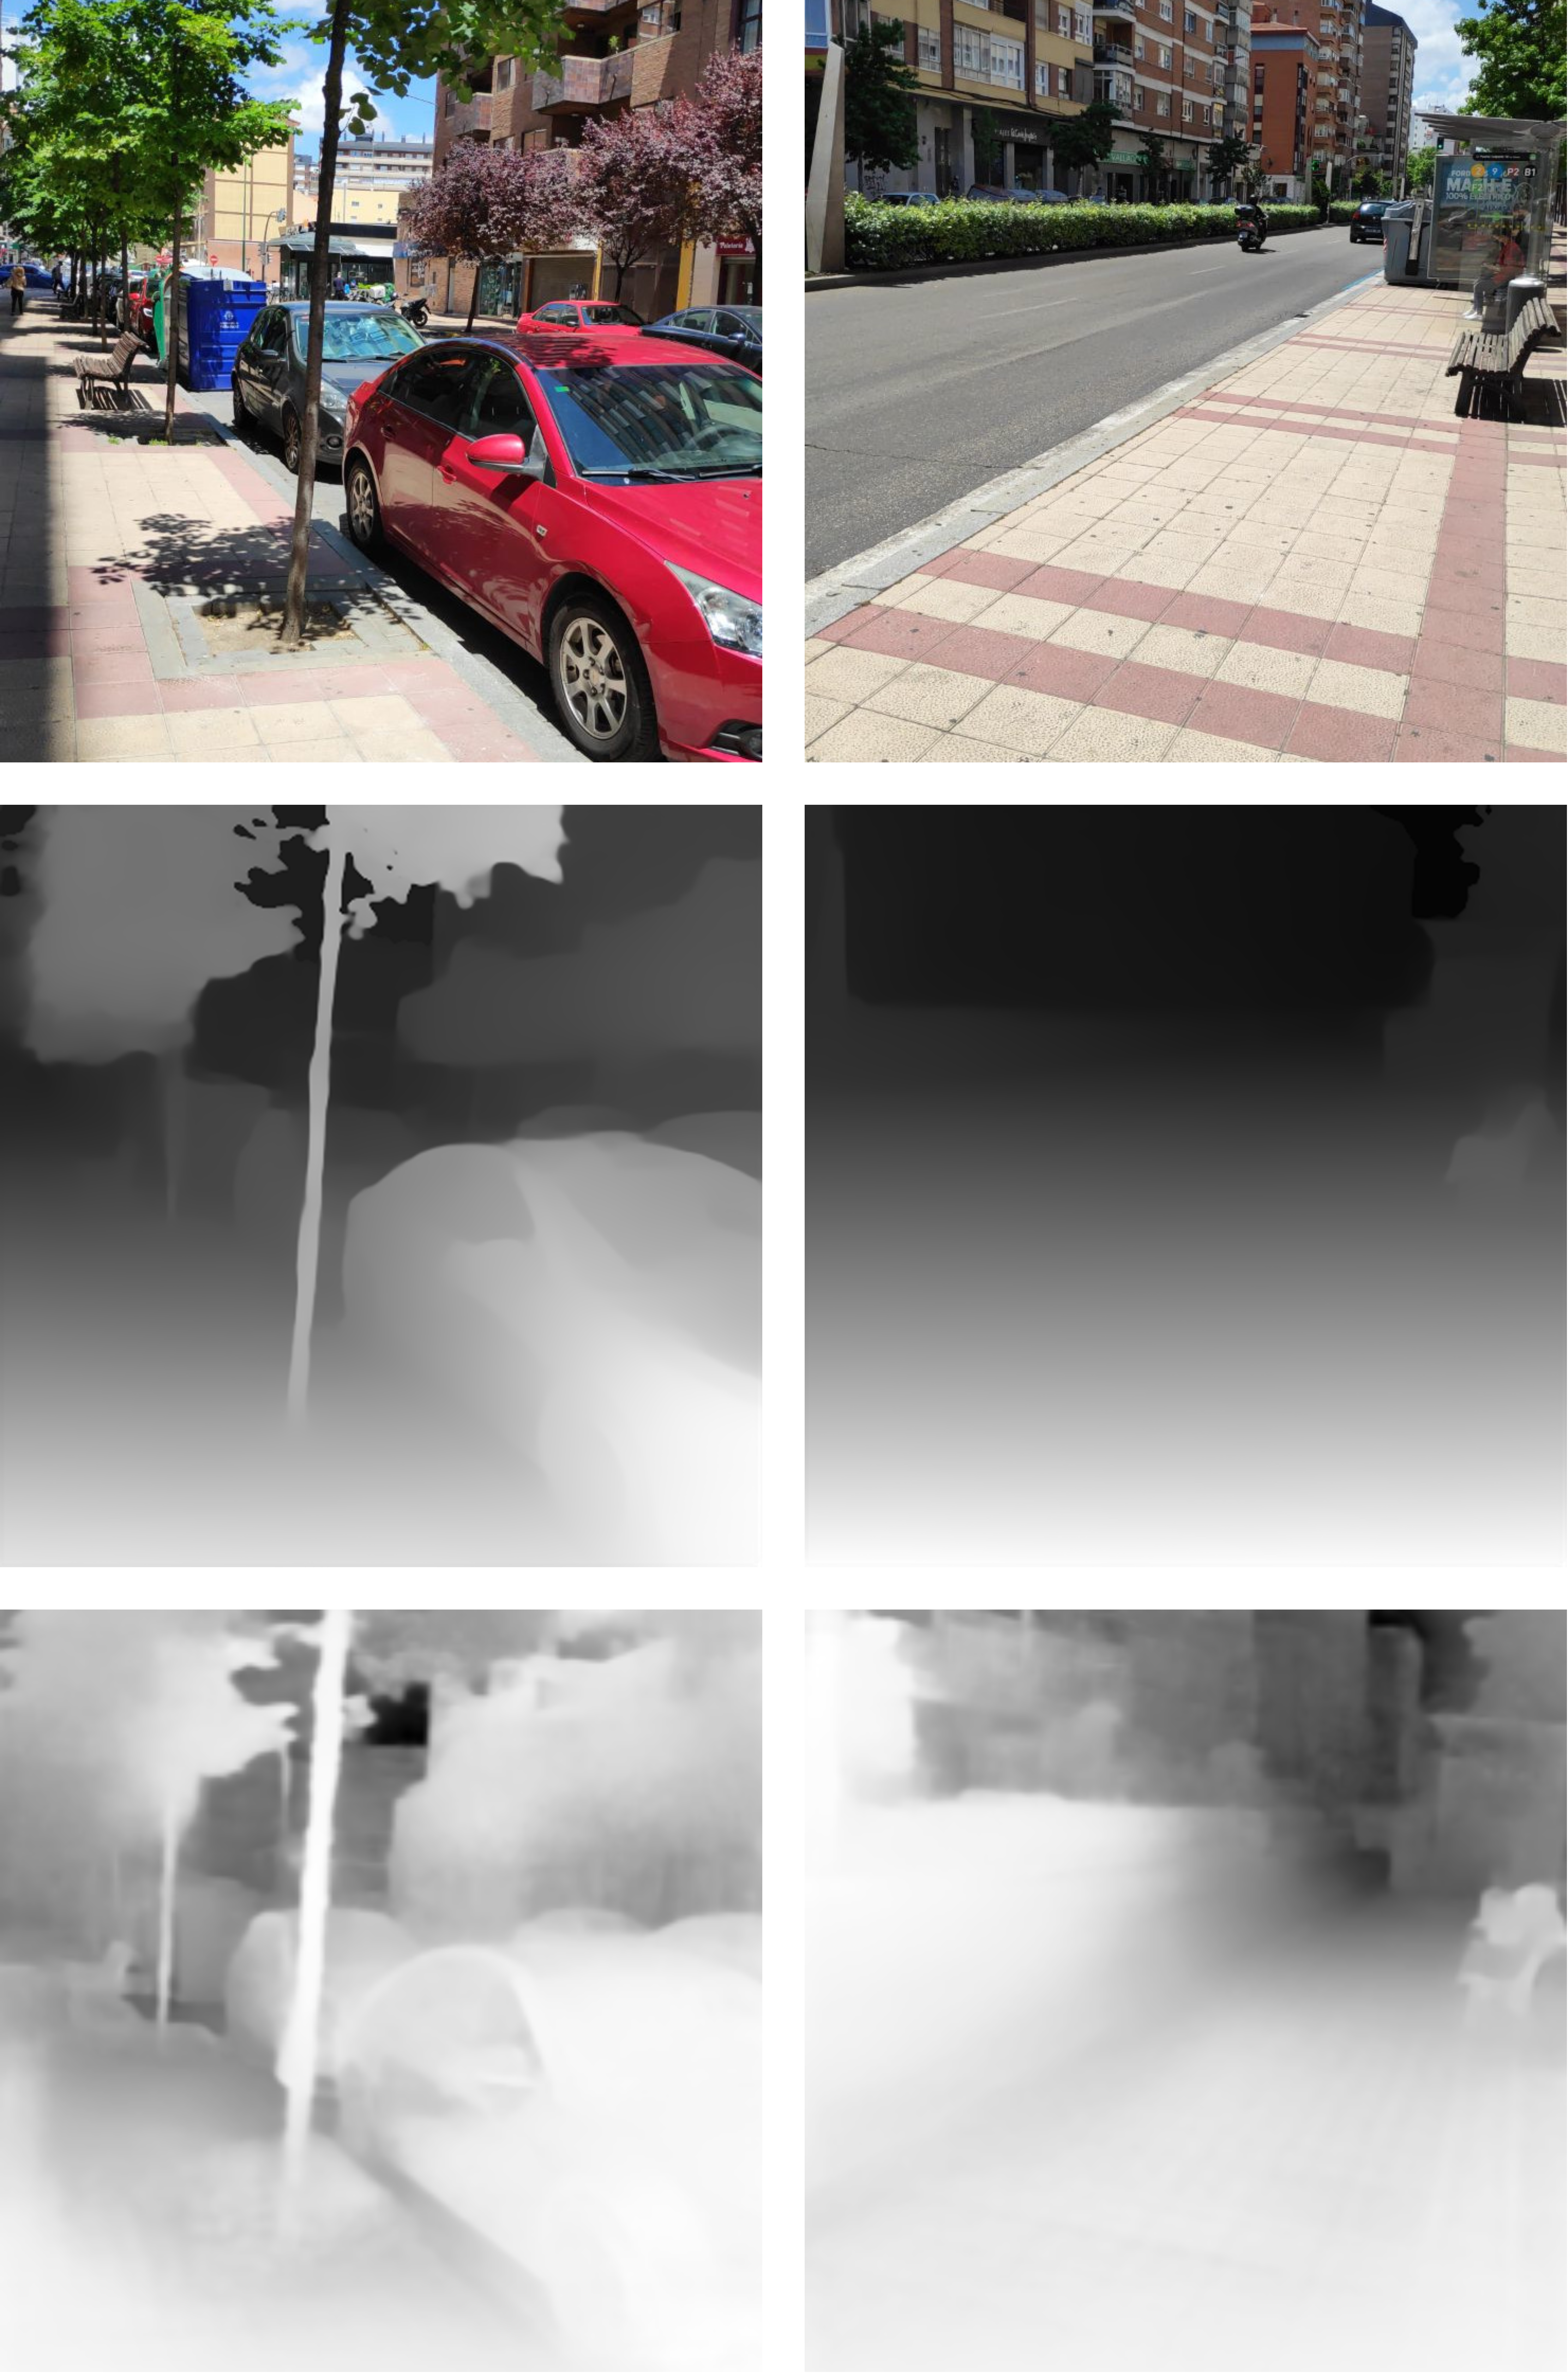
\includegraphics[width=0.9\linewidth]{imagenes/resultados2.png} 
% \captionsetup{width=.8\linewidth}
% \caption{Resultados de \textit{DPT} y \textit{AdaBins} en dos imágenes. Primera fila - imágenes de entrada, segunda fila - resultados \textit{DPT}, tercera fila - resultados \textit{AdaBins}.}
% \label{fig:resultados-anexo2}
% \end{figure}






% \clearpage
%\section{WIP: Texto de dataset mix5 y mix6}\label{unk}
%DPT parece que no está preparado para pasarse a onnx (o sí https://github.com/isl-org/DPT/issues/42), una de las opciones sería reescribir el modelo (probablemente simplificado) y reentrenar. Se describe a continuación los dataset empleados, reentrenar no parece muy viable. Otra opción que se podría explorar es destilar el modelo de alguna forma. También se puede leer los data efficient transformers de facebook a ver si reducen la necesidad de emplear tantisimas imágenes. Otra opción (si la implementación de Adabins está hecha orientada a onnx, sería usar solamente adabins y hacer todo el tfm con esa arquitectura).
%
%El dataset de profundidad que se usa para entrenar DPT (MIX6) es una ampliación de MIX5, presentado en \url{https://arxiv.org/abs/1907.01341}, el cual incluía los datasets:
%\begin{itemize}
%\item ReDWeb (\url{https://sites.google.com/site/redwebcvpr18/})
%\item DIML (\url{https://dimlrgbd.github.io/})
%\item 3D Movies (\url{https://github.com/isl-org/MiDaS/issues/13}) (\url{https://github.com/isl-org/MiDaS/issues/24}) el material complementario no está en el paperv3, ver v2 \url{https://arxiv.org/pdf/1907.01341v2.pdf}
%\item MegaDepth (\url{https://www.cs.cornell.edu/projects/megadepth/})
%\item WSVD (este también es un jaleo hacerlo \url{https://sites.google.com/view/wsvd/home} ; \url{https://github.com/aycatakmaz/wsvd_dataset_loader}) se descargan vídeos de youtube y se calcula, parecido a 3d movies, parece más automatizado.
%\end{itemize}
%
%Para el artículo de DPT, se incluyen cinco dataset más para conseguir MIX6:
%\begin{itemize}
%\item TartanAir (\url{https://theairlab.org/tartanair-dataset/})
%\item HRWSI (\url{https://github.com/KexianHust/Structure-Guided-Ranking-Loss})
%\item ApolloScape (\url{http://apolloscape.auto/stereo.html})
%\item BlendedMVS (\url{https://github.com/YoYo000/BlendedMVS})
%\item IRS (\url{https://github.com/HKBU-HPML/IRS})
%\end{itemize}
%
%Estos datasets se usan para entrenamiento solamente. Para el test, se usan los siguientes datasets: 
%
%\begin{itemize}
%\item DIW (\url{http://www-personal.umich.edu/~wfchen/depth-in-the-wild/})
%\item ETH3D (\url{https://www.eth3d.net/datasets})
%\item Sintel (\url{http://sintel.is.tue.mpg.de/about})
%\item KITTI (\url{https://stackoverflow.com/questions/63512296/kitti-eigen-split} - \url{http://www.cvlibs.net/datasets/kitti/eval_depth.php?benchmark=depth_prediction})
%\item NYU (\url{https://cs.nyu.edu/~silberman/datasets/nyu_depth_v2.html})
%\item TUM (\url{https://vision.in.tum.de/data/datasets/rgbd-dataset}). 
%Tanto en el paper de DPT como en el paper de MiDas (versión anterior y convolucional de DPT (\url{https://github.com/isl-org/MiDaS})).
%\end{itemize}








%\section{Evaluación y pruebas}\label{resultados}
%% \todo[inline]{Hablar de las pruebas que se han hecho, valorar CPU GPU y TPU?. Comparar con los resultados que proporcionan los papers si es que los proporcionan.}
%% \todo[inline]{Hacer un experimento de pruning como el de Learning both weights and connections for efficient neural networks. La visualización de la distribución de los pesos antes y después del pruning también es muy interesante. (TFM)}
%% \todo[inline]{Hacer experimento de ablación para ver que partes corresponden a un mayor incremento/decremento de la velocidad/accuracy. (TFM)}
%% \todo[inline]{Redactar todo esto mejor}
%
%Para tener una estimación de cuánto tardan en realizar inferencia los modelos de estimación de profundidad monocular no eficientes que emplean \textit{transformers} y aprendizaje supervisado (expuestos en la sección \hyperref[aprendizaje-supervisado]{Aprendizaje supervisado}), se llevan a cabo una serie de pruebas en GPU y CPU. Siguiendo la metodología expuesta en \cite{visiontransformersDPT}, se mide el tiempo de inferencia media en 400 imágenes de 384x384 píxeles. Estas pruebas, se llevan a cabo tanto como para \textit{Dense Prediction Transformers} como para \textit{AdaBins} (Tabla \ref{tab:resultados-inferencia}). Además de estas pruebas de velocidad, también se han realizado pruebas sobre imágenes propias, algunas de las cuales están disponibles en el \hyperref[anexo1]{Anexo 1}. 
%% \todo{Incluir imágenes}.
%%Se obtienen resultados bastante razonables considerando que se emplean gráficas diferentes.\\
%
%\begin{table}[H]
%\centering
%\begin{tabular}{cccccc}
%\toprule
%             & \multicolumn{2}{c}{Inferencia (ms)} & \multicolumn{2}{c}{FPS} &           \\ 
%Prueba       & DPT  & AdaBins                      & DPT  & AdaBins          & Hardware  \\ \midrule
%Paper DPT    & 38   & -                            & 26.3 & -                & RTX 2080 (GPU) \\
%Propia   & 41   & 105                          & 24.5 & 9.52             & RTX 3070 (GPU) \\
%Propia (Colab) & 60   & 164                            & 16.7 & 6.08                & Tesla T4 (GPU)\\
%Propia    & 1675 & 2008                         & 0.60 & 0.50             & AMD\textsuperscript{\textregistered} Ryzen 7 3800x (CPU) \\ \bottomrule
%\end{tabular}
%\caption{Resultados de tiempos de inferencia con DPT y AdaBins}
%\label{tab:resultados-inferencia}
%\end{table}